

%%%%%%%%%%%%%%%%%%%%%%%%%%%%%%%%
%-------------- version with R(S) only starts here ----------
%%%%%%%%%%%%%%%%%%%%%%%%%%%%%%%%


%%% For double-blind review submission, w/o CCS and ACM Reference (max 
%%%submission space)
%\documentclass[sigplan,review,anonymous,10pt]{acmart}\settopmatter{printfolios=true,printccs=false,printacmref=false}
%%% For double-blind review submission, w/ CCS and ACM Reference
%%\documentclass[sigplan,review,anonymous]{acmart}\settopmatter{printfolios=true}
%%% For single-blind review submission, w/o CCS and ACM Reference (max 
%%%submission space)
%%\documentclass[sigplan,review]{acmart}\settopmatter{printfolios=true,printccs=false,printacmref=false}
%%% For single-blind review submission, w/ CCS and ACM Reference
%%\documentclass[sigplan,review]{acmart}\settopmatter{printfolios=true}
%%% For final camera-ready submission, w/ required CCS and ACM Reference
%%\documentclass[sigplan]{acmart}\settopmatter{}
%
%\usepackage{soul}
%
%\usepackage{color, colortbl}
%
%%\usepackage{booktabs} % For formal tables
%%\documentclass{article}
%%\usepackage{floatrow}
%\usepackage{rotating}
%\usepackage{graphicx}
%\usepackage{multirow}
%%\usepackage[dvipsnames]{xcolor}
%\usepackage{amsfonts}
%\usepackage{amsmath}
%\usepackage{amssymb}
%\usepackage{mathtools}
%\usepackage{wrapfig}
%\usepackage{listings}
%\usepackage{graphicx}
%\usepackage{caption}
%\usepackage{tabularx}
%%\usepackage{amsthm}
%%\usepackage[section]{placeins}
%\usepackage{enumitem}
%%\usepackage[a4paper, total={7in, 10.5in}]{geometry}
%\usepackage[font={small}]{caption}
%%\usepackage[font={bf,sf,small}]{caption}
%%\usepackage[linesnumbered,ruled]{algorithm2e}
%\usepackage{algpseudocode}
%\captionsetup{labelfont=bf,textfont=bf}
%\usepackage[font={bf,sf,scriptsize}]{subfig} 
%\usepackage{amsthm}
%
%%
%%\usepackage[utf8]{inputenc}
%%\usepackage{url}
%%\usepackage{amsmath,amsthm,amssymb,amsfonts}
%\usepackage{algorithm}
%\usepackage{algpseudocode}
%\usepackage{algorithmicx}
%%\usepackage{graphicx}
%%\usepackage{caption}
%%\usepackage[thinlines]{easytable}
%%\usepackage{pdfpages}
%%\usepackage{fancyhdr}
%%\usepackage{booktabs}
%%\usepackage{footnote}
%%\usepackage{footmisc}
%%\usepackage{mathtools}
%%\usepackage{multirow}
%%%\usepackage{siunitx}
%%%\usepackage{booktabs}
%%%\usepackage{blindtext}
%%%\usepackage[pdfencoding=auto,psdextra]{hyperref}
%%
%%\fancyhf{}
%%\renewcommand{\headrulewidth}{0pt}
%%\renewcommand{\footrulewidth}{0pt}
%%
%%\DeclarePairedDelimiter\abs{\lvert}{\rvert}
%%
%%\makeatletter
%%\let\oldabs\abs
%%\def\abs{\@ifstar{\oldabs}{\oldabs*}}
%%\makeatother
%%\def\E{\mathbb{E}}
%%
%%\makeatletter
%%\g@addto@macro \normalsize {%
%%	\setlength\abovedisplayskip{5pt plus 2pt minus 2pt}%
%%	\setlength\belowdisplayskip{5pt plus 2pt minus 2pt}%
%%}
%%\makeatother
%
%
%\renewcommand{\algorithmicrequire}{\textbf{Input:}}
%\renewcommand{\algorithmicensure}{\textbf{Output:}}
%
%\newcommand\numberthis{\addtocounter{equation}{1}\tag{\theequation}}
%\def\NoNumber#1{{\def\alglinenumber##1{}\State #1}\addtocounter{ALG@line}{-1}}
%
%
%
%%\usepackage[demo]{graphicx}
%%\setlength{\footskip}{15pt}
%%\usepackage[utf8]{inputenc}
%%\usepackage[english]{babel}
%\newtheorem{theorem}{Theorem}[section]
%\newtheorem*{corollary*}{Corollary}
%\newtheorem{corollary}{Corollary}[theorem]
%%\newtheorem{lemma}[theorem]{Lemma}
%\newcommand\todo[1]{\textcolor{red}{#1}}
%\newcommand\greg[1]{\textcolor{blue}{[Greg: #1]}}
%\newcommand\toskip[1]{\textcolor{green}{[possibly to skip: #1]}}
%\newcommand\mac[1]{\textcolor{red}{[Mac: #1]}}
%
%\newcommand*\diff{\mathop{}\!\mathrm{d}}
%\newcommand*\Diff[1]{\mathop{}\!\mathrm{d^#1}}
%
%\DeclareMathOperator*{\argmax}{arg\,max}
%\DeclareMathOperator*{\argmin}{arg\,min}
%
%%  \lstset{language=C,
%%    keepspaces=true,
%%    frame=tb,
%%    basicstyle=\ttfamily,
%%    columns=fixed,
%%    morekeywords={enddo},
%%    mathescape}
%
%\definecolor{darkgrey}{RGB}{70,70,70}
%\definecolor{lightgrey}{RGB}{200,200,200}
%
%\lstset{language=C,
%	escapechar=|,
%	keepspaces=false,
%	frame=tb,
%	framexleftmargin=1.5em,
%	basicstyle=\tt\scriptsize,
%	columns=fixed,
%	%otherkeywords={enddo,forall,bool,true,false, int64_t, MPI_Op, in, 
%	%parallel, function},
%	otherkeywords={enddo,end,forall,bool,true,false, int64_t, MPI_Op, 
%		function},
%	tabsize=2,
%	breaklines=true,
%	captionpos=b,
%	%aboveskip=-1.5em,
%	%belowskip=-0.5em,
%	numbers=left,
%	xleftmargin=1.5em,
%	keywordstyle=\bfseries\color{black!400!black},
%	stringstyle=\color{orange},
%	commentstyle=\color{darkgrey},
%	numberstyle=\scriptsize,numbersep=3pt,mathescape}
%
%
%\usepackage[font={bf,sf,scriptsize}]{caption}
%%\usepackage[font={bf,sf,scriptsize}]{subfig}
%
%\usepackage{cleveref}
%\usepackage[utf8]{inputenc}
%\crefname{section}{§}{§§}
%\Crefname{section}{§}{§§}
%
%\newtheorem{defn}{Definition}
%\newtheorem{thm}{Theorem}
%\newtheorem{clm}{Claim}
%\newtheorem{crl}{Corollary}
%\newtheorem{lma}{Lemma}
%%\newtheorem{proof}{Proof}
%%\newtheorem*{proof*}{Proof}
%\newtheorem{observation}{Observation}
%
%\newcommand{\macb}[1]{\textbf{\textsf{#1}}}
%
%\DeclareSymbolFont{matha}{OML}{txmi}{m}{it}% txfonts
%\DeclareMathSymbol{\varS}{\mathord}{matha}{83}
%
%\acmConference[PPoPP'19]{ACM SIGPLAN Annual Symposium on Principles and 
%	Practice of Parallel Programming}{February 16--20, 2019}{Washington DC, USA}
%% \acmYear{}
%% \acmISBN{} 
%% \acmDOI{}
%\startPage{1}
%
%%% Copyright information
%%% Supplied to authors (based on authors' rights management selection;
%%% see authors.acm.org) by publisher for camera-ready submission;
%%% use 'none' for review submission.
%\setcopyright{none}
%%\setcopyright{acmcopyright}
%%\setcopyright{acmlicensed}
%%\setcopyright{rightsretained}
%%\copyrightyear{2018}           %% If different from \acmYear
%
%%% Some recommended packages.
%\usepackage{booktabs} 
%\usepackage{makecell}
%\hypersetup{draft}
%
%\usepackage{pifont}
%
%\begin{document}
%	
%	%% Title information
%	
%	\title[I/O-Optimal Dimensionless Matrix 
%	Multiplication]{\vspace{-1em}Breaking 
%		The 
%		Monopoly of Dimensions: Towards I/O-Optimal Matrix Multiplication}
%	
%	
%	\author{First1 Last1}
%	\authornote{with author1 note}          %% \authornote is optional;
%	%% can be repeated if necessary
%	\orcid{nnnn-nnnn-nnnn-nnnn}             %% \orcid is optional
%	\affiliation{
%		\position{Position1}
%		\department{Department1}              %% \department is recommended
%		\institution{Institution1}            %% \institution is required
%		\streetaddress{Street1 Address1}
%		\city{City1}
%		\state{State1}
%		\postcode{Post-Code1}
%		\country{Country1}                    %% \country is recommended
%	}
%	\email{first1.last1@inst1.edu}          %% \email is recommended
%	
%	%% Author with two affiliations and emails.
%	\author{First2 Last2}
%	\authornote{with author2 note}          %% \authornote is optional;
%	%% can be repeated if necessary
%	\orcid{nnnn-nnnn-nnnn-nnnn}             %% \orcid is optional
%	\affiliation{
%		\position{Position2a}
%		\department{Department2a}             %% \department is recommended
%		\institution{Institution2a}           %% \institution is required
%		\streetaddress{Street2a Address2a}
%		\city{City2a}
%		\state{State2a}
%		\postcode{Post-Code2a}
%		\country{Country2a}                   %% \country is recommended
%	}
%	\email{first2.last2@inst2a.com}         %% \email is recommended
%	\affiliation{
%		\position{Position2b}
%		\department{Department2b}             %% \department is recommended
%		\institution{Institution2b}           %% \institution is required
%		\streetaddress{Street3b Address2b}
%		\city{City2b}
%		\state{State2b}
%		\postcode{Post-Code2b}
%		\country{Country2b}                   %% \country is recommended
%	}
%	\email{first2.last2@inst2b.org}         %% \email is recommended
%	
%	
%	
%	\appendix
%	
%	
%	\section{I/O Lower Bounds for Arbitrary CDAGs}
%	\label{sec:introIO}
%	In this section we shortly introduce a general mathematical machinery we 
%	use to 
%	proof 
%	the I/O optimality of COMM. We extend Lemma~\ref{lma:spartlemma} by 
%	Hong and 
%	Kung~\cite{redblue}, which provides a method to find an I/O lower bound for 
%	a 
%	given CDAG. This lemma, however, does not give a tight bound, as it 
%	overestimates a \emph{reuse set} size (cf. 
%	Lemma~\ref{lma:reuse}). Our key result here, Lemma~\ref{lma:reuse} 
%	allows us to derive a constructive proof of a tighter I/O lower bound for a 
%	sequential execution of MMM CDAG~(\cref{sec:seqOptimality}). We use this 
%	result 
%	in~(\cref{sec:parOptimality}) to prove the parallel I/O optimality of COMM.
%	
%	Our method heavily relies on a red-blue pebble game 
%	(Definition~\ref{df:redbluegame}) 
%	and an $S$-partition abstractions (Definition~\ref{df:s-partition}) 
%	introduced 
%	by Hong and Kung.
%	
%	\subsection{Red-Blue Pebble Game}
%	A red-blue pebble game is an abstraction modeling an execution of an 
%	algorithm 
%	in a two-level memory structure with a 
%	small-and-fast
%	as well as large-and-slow memory. A red (or a blue) pebble placed on a 
%	vertex 
%	of a CDAG denotes that this data is inside a fast (or slow) memory.  It is 
%	a 
%	powerful tool, extensible to
%	arbitrarily many memory levels~\cite{redblueHierarchy}, that was used to 
%	derive
%	lower bounds for algorithms such as sorting or FFT~\cite{redblue}. 
%	
%	\macb{Intuition}
%	%
%	In the red-blue pebble game, a red (or blue) pebble placed on a vertex 
%	denotes 
%	that its value is inside the fast (or slow) memory.
%	%
%	%A computation of a 
%	%CDAG starts with placing
%	%certain \emph{pebbles} on its input vertices\greg{changed "certain 
%	%number of pebbles" to "certain pebbles". The first one was just wrong.}, 
%	%which 
%	%corresponds to 
%	%loading the
%	%data from the slow to the fast memory. 
%	%
%	The actual computation (referred to as
%	\emph{pebbling}) is a series of allowed moves (e.g., moving a pebble from 
%	one
%	vertex to another) that correspond to load, store, compute, or
%	freeing-memory operations.
%	%
%	The \emph{I/O cost of a computation} is the number of pebble moves that
%	correspond to loads and stores between the slow and the fast memory; 
%	finding 
%	the pebbling that minimizes
%	this cost is PSPACE-complete~\cite{redbluecomplete, pebblegameregister}. 
%	
%	\begin{defn}[Red-Blue Pebble Game~\cite{redblue}] \label{df:redbluegame}
%		Let $G = (V,E)$ be a CDAG. 
%		In the initial/terminal configuration, only inputs/outputs of the CDAG 
%		have
%		blue pebbles.
%		%
%		There can be at most $S$ red pebbles used. A complete CDAG computation 
%		is a
%		sequence of moves that lead from the initial to the terminal pebble
%		configuration.
%		%
%		The allowed moves are as follows: \ding{172} placing a red pebble on 
%		any 
%		vertex
%		with a blue pebble (load), \ding{173} placing a blue pebble on any 
%		vertex 
%		with 
%		a red
%		pebble (store), \ding{174} placing a red pebble on a vertex whose 
%		parents 
%		have 
%		all red
%		pebbles (compute), \ding{175} removing any pebble (red or blue) from 
%		any 
%		vertex 
%		(freeing memory).
%	\end{defn}
%	
%	An I/O optimal execution of a CDAG corresponds to a sequence of moves 
%	(called 
%	\emph{pebbling} of a graph) which minimizes load \ding{172} and store 
%	\ding{173} moves.
%	
%	\macb{Connections to MMM}
%	%
%	For a CDAG of MMM, an example pebbling moves include placing red pebbles on 
%	some vertices
%	corresponding to elements of matrices $A$ and $B$ (load operations), 
%	placing red
%	pebbles on the corresponding elements of $C$ (compute), removing red
%	pebbles from the loaded inputs (freeing memory) and placing blue pebbles on 
%	the
%	computed elements of $C$ (store). 
%	
%	\subsection{$S$-Partitions}
%	
%	
%	The notion of an \emph{$S$-partition} facilitates deriving lower bounds on 
%	the
%	I/O computation cost~\cite{redblue}. Here, one divides a given CDAG into
%	consecutive \emph{subcomputations}, each of which requires at least $S$ 
%	load 
%	and store
%	operations. The key element in more straightforward
%	lower bound proofs is to analytically bound the size (vertex count) of
%	the largest subcomputation, given its input and output size (i.e., the 
%	number
%	of vertices outside (inside) the subcomputation that have a child inside
%	(outside) of it). 
%	%
%	%\macb{Intuition}
%	%
%	%Intuitively, the $S$-partition technique may be seen as a generalization of
%	%the Loomis-Whitney inequality~\cite{loomisWhitney}, which is used in linear
%	%algebra for bounding the amount of I/O~\cite{loomisApplied}: both 
%	%techniques
%	%aim at finding the optimal surface (communication) to volume (computation)
%	%ratio in a given setting. 
%	%
%	%$S$-partition was used to derive the first I/O bounds for matrix
%	%multiplication, FFT, or odd-even transposition sorting~\cite{redblue}.
%	%
%	%\macb{Details}
%	%
%	Formally:
%	
%	\begin{defn}[$S$-partition of a CDAG~\cite{redblue}] \label{df:s-partition}
%		%
%		Let $G = (V,E)$ be a CDAG. An $S$-partition of $G$ is a collection 
%		$\{V_1, 
%		...,
%		V_h\}$ of $h$ subcomputations of $ V$ such that: \ding{192} $V_i \cap 
%		V_j
%		=\emptyset\ $ and $\bigcup_{i=1}^{h} V_i=V$ for any $1 \le i,j \le h$,
%		\ding{193} $\forall i\quad |Dom(V_i)| \le S$, \ding{194} $\forall i\quad
%		|Min(V_i)| \le S$, and \ding{195} there is no cyclic dependence between
%		subcomputations.
%		%   
%		% \begin{itemize} \item $\forall_{1 \le i,j \le h}\quad V_i \cap V_j
%		% =\emptyset\ $ and $\ \bigcup_{i=1}^{h} V_i=V$ \item $\forall i\quad
%		% |Dom(V_i)| \le S$ \item $\forall i\quad |Min(V_i)| \le S$ \item there 
%		%is 
%		%no
%		% cyclic dependence between subcomputations.  \end{itemize}
%		%
%	\end{defn}
%	
%	$Dom(V_i) \not \subset V_i$ is the \emph{dominator set}: a set of vertices 
%	such 
%	that
%	every path from an input of the CDAG to a vertex in $V_i$ contains some 
%	vertex in in
%	$Dom(V_i)$.
%	%
%	$Min(V_i) \subset V_i$ is the \emph{minimum set} of $V_i$: it contains 
%	vertices
%	that do not have any children in $V_i$. 
%	%
%	%Throughout this paper, we will use \emph{subset} and \emph{subcomputation}
%	%interchangeably, to emphasize its interpretation in the context of 
%	%scheduling. 
%	%
%	Finally, $H(S)$ is the cardinality of the smallest valid $S$-partition of a
%	given CDAG.
%	
%	We use a symbol $\mathcal{S}(S) = \{V_1, \dots , V_h\}$ to 
%	denote an $S$-partition. 
%	%
%	% there is a
%	%lower bound on the cardinality of a valid $S$-partition.  We denote this
%	%minimal number of vertex sets with a dedicated symbol $H(S)$.
%	
%	\macb{Connections to MMM}
%	%
%	In MMM, a subcomputation $V_i$ is a calculation of partial sums of $C$ that 
%	can
%	be computed with at most $S$ elements of $A$ and $B$, and that contributes 
%	to
%	at most $S$ outputs. Those elements from $A$ and $B$, as well as previous
%	values of $C$ being updated, form $Dom(V_i)$. Then, $Min(V_i)$ corresponds 
%	to
%	the result of this subcomputation (cf.~
%	Figure~\ref{fig:iterationSpace}). $H(S)$ denotes 
%	the
%	number of such subsets required to calculate the final result. Assuming 
%	that 
%	each subcomputation computes the same number of partial results 
%	$\forall_{i,j}|V_i| = |V_j|$, and observing the total number of partial 
%	results 
%	$|V| = mnk$, we have $H(S) = \frac{mnk}{V_i}$.
%	% (geometrically
%	%\mac{what does geometrically mean?}, \mac{the} number of subsets require
%	%\mac{required} to fill the entire 3D iteration space \mac{what 3D space? 
%	%was
%	%*never* defined or even mentioned... Already complained. I think the best 
%	%place
%	%is the background subsection dedicated to MMM. It can be very brief (1-2 
%	%sentences)}).
%	
%	\subsection{Existing General I/O Lower Bound}
%	\label{sec:spartProof}
%	
%	%\greg{Observation: 2S-partition reduces scheduling problem (P-space) 
%	%to 
%	%partitioning problem (NP-complete)?}
%	%\greg{...... UPDATE: I don't show here the proof of NP-completeness 
%	%of 
%	%S-partitioning. Too much space. Better skip this observation}
%	
%	We now cite a \emph{general} lower bound on the cost of \emph{any} I/O
%	computation~\cite{redblue} and sketch the proof, which is the basis for our
%	\emph{tighter general} bound on the I/O cost (Lemma~\ref{lma:reuse}).
%	
%	\macb{Intuition}
%	%
%	The key notion in the existing bound is to use $2S$-partitions for a given 
%	fast
%	memory size~$S$.
%	%
%	For some subcomputation $V_i$, if $|Dom(V_i)| = 2S$ vertices, then at most 
%	$S$
%	of them could contain a red pebble before $V_i$ begins.  Thus, at least $S$
%	additional pebbles need to be loaded from the memory.  The similar argument
%	goes for $Min(V_i)$. Therefore, knowing the lower bound on the number of 
%	sets
%	$V_i$ in a valid \emph{$2S$-partition}, together with the observation that 
%	each
%	$V_i$ performs at least $S$ I/O operations, we have:
%	%
%	%  a \emph{$2S$-partitioning} of the
%	%graph. Thus, each subcomputation $V_i$ requires $2S$ input elements (the
%	%dominator set) to perform the computation. Because at most $S$ elements 
%	%could
%	%already be in the fast memory from the previous computation (recall that 
%	%the
%	%size of the fast memory is $S$), the remaining $S$ elements have to be 
%	%loaded
%	%from the slow memory. 
%	%
%	%Similarly, because $V_i$ has $2S$ output elements (the minimum set), but 
%	%only 
%	%$S$
%	%can be immediately consumed by the next computation, remaining $S$ elements
%	%have to be stored in the slow memory. By finding the minimum number of 
%	%valid
%	%$S$-partition subsets \mac{why S and not 2S? This sentence seems completely
%	%detached from the previous text}, we derive the I/O lower bound:
%	
%	\begin{lma}[Lower bound on the number of I/Os~\cite{redblue}]
%		%
%		The minimal number $Q$ of I/O operations for any valid execution of a 
%		CDAG 
%		of
%		any I/O computation is bounded by
%		
%		\begin{equation}
%		\label{eq:redbluebound}
%		Q \ge S \cdot (H(2S) - 1)
%		\end{equation}
%		%
%	\end{lma}
%	
%	\macb{Details}
%	%
%	% We now sketch the original proof, as we use it as a basis for our
%	% Lemma~\ref{lma:reuse}, which gives a tighter I/O bound.
%	%
%	Assume that we know the optimal schedule of the CDAG. Divide the computation
%	into $h$ consecutive subcomputations $V_1, V_2, ..., V_h$, such that during 
%	the
%	execution of $V_i$, $i < h$, there are exactly $S$ I/O operations, and in 
%	$V_h$
%	there are at most $S$ operations. Now, for each $V_i$, we define two 
%	subsets of
%	$V$, $V_{R,i}$ and $V_{BR,i}$.
%	%
%	%\begin{enumerate}[leftmargin=1.5em]
%	%
%	$V_{R,i}$ contains vertices that have red pebbles placed on them just before
%	$V_i$ begins.
%	%
%	$V_{BR,i}$ contains vertices that have blue pebbles placed on them just 
%	before
%	$V_i$ begins, and have red pebbles placed on them during $V_i$.
%	%
%	% \end{enumerate}
%	%
%	% \noindent
%	%
%	% Then, one can derive the following observations:
%	%
%	Using these definitions, we have: \ding{182} $V_{R,i} \cup V_{BR,i} =
%	Dom(V_i)$, \ding{183} $|V_{R,i}| \le S$, \ding{184} $|V_{BR,i}| \le S$, and
%	\ding{185} $|V_{R,i} \cup V_{BR,i}| \le |V_{R,i}| + |V_{BR,i}| \le 2S$.
%	% 
%	% \begin{enumerate}
%	%   %
%	%   \item $V_{R,i} \cup V_{BR,i} = Dom(V_i)$
%	%   %
%	%   \item $|V_{R,i}| \le S$
%	%   %
%	%   \item $|V_{BR,i}| \le S$
%	%   %
%	%   \item $|V_{R,i} \cup V_{BR,i}| \le |V_{R,i}| + |V_{BR,i}| \le 2S$
%	%   %
%	% \end{enumerate}
%	% 
%	We define similar subsets $W_{BR,i}$ and $W_{R,i}$ for the minimum set 
%	$Min(V_i)$.  $W_{BR,i}$ contains all vertices in $V_i$ that have a blue 
%	pebble placed on them during $V_i$, and  $W_{R,i}$ contains all vertices in 
%	$V_i$ that have a red pebble at the end of $V_i$. By the definition of 
%	$V_i$, 
%	$W_{BR,i} \le S$, by the constraint on the red pebbles, we have $W_{R,i} 
%	\le 
%	S$, and by te definition of the minimum set,$Min(V_i) \subset W_{R,i} \cup 
%	W_{BR,i}$.
%	%
%	Finally, by Definition~\ref{df:s-partition}, $V_1, V_2, ..., V_h$ form a 
%	valid
%	$2S$-partition of the CDAG. 
%	
%	% We now proceed to show how we can tighten this bound by tightening the 
%	%bound
%	% on the set $V_{R,i}$, that is, the data reuse between the computations. 
%	
%	
%	\subsection{Tighter General I/O Lower Bounds}
%	\label{sec:seq-proof}
%	
%	
%	\subsubsection{Data Reuse}
%	\label{sec:datareuse}
%	
%	A more careful look at the sets $V_{R,i}$ and  $V_{BR,i}$
%	allows us to 
%	refine the bound on the number of I/O operations on a CDAG. By its 
%	definition,  
%	$V_{BR,i}$ is a set of vertices on which we perform move \ding{172} 
%	(load).  
%	On the other hand, $V_{R,i}$ is the set of vertices that were already 
%	computed 
%	(red-pebbled) during some $V_j, j < i$, and are reused during $V_i$ (the 
%	move 
%	\ding{172} is not needed).  
%	We call $V_{R,i}$ a \emph{reuse set} of $V_i$. 
%	The trivial bounds on $V_{R,i}$ is
%	$V_{R,i} \le S$, but if one can show that 
%	$\exists_{R(S) 
%		\in \mathbb{Z}}: 
%	\forall_i: V_{R,i} \le R(S) < S$, we can use $R(S)$  to tighten a 
%	bound 
%	on 
%	$Q$. We call $R(S)$ a \emph{maximum reuse} of 
%	a CDAG.
%	
%	
%	\subsubsection{Reuse-based Lemma}
%	
%	%\greg{Just one sentence that we derive data movement optimal 
%	%schedule starting 
%	%from I/O optimal (sequential) schedule}
%	%
%	%\greg{updated}
%	
%	We now enhance the general I/O lower bound \emph{by tightening the bound on 
%	the
%		set $V_{R,i}$}, that is, the \emph{data reuse between the computations}
%	%
%	bounds. 
%	%
%	%\subsection{2S-partition, S-partition and data reuse}
%	% \subsubsection{Tighter Sequential Bounds with Explicit Data Reuse}
%	%
%	% Specifically, we modify the original proof and show that finding the 
%	%minimum
%	% number of subsets in an $S$-partition (instead of a $2S$-partition), 
%	%together 
%	% with the bound on data reuse $V_{R,i}$ gives
%	% tighter lower bounds.
%	%
%	%\macb{Intuition}
%	%
%	%
%	Our main result in this section is as follows:
%	
%	\begin{lma}
%		\label{lma:reuse}
%		%
%		The minimal number $Q$ of I/O operations for any valid execution of a 
%		CDAG 
%		$\ G=(V,E)$ is bounded by  
%		
%		\vspace{-0.5em}
%		\begin{equation}
%		%
%		Q \ge (S - R(S)) \cdot (H(S) - 1)
%		%
%		\label{eq:reusebound} \end{equation}
%		\vspace{-0.5em}
%		
%		\noindent
%		$R(S)$ is the maximum reuse and $T(S)$ is the minimum store 
%		size~(\cref{sec:datareuse}).
%		Moreover: 
%		
%		\vspace{-0.5em}
%		\begin{equation}\label{eq:reusebound-pmax}
%		H(S) \ge \frac{|V|}{|V_{max}|}
%		\end{equation}
%		\vspace{-0.5em}
%		
%		\noindent
%		where $V_{max} = \argmax_{V_i \in \mathcal{S}}|V_i|$ is 
%		the largest
%		subset of vertices in $\mathcal{S}(S)$.
%		
%		% \begin{equation}
%		% H(S) \ge \frac{|V|}{|P_{max}|}
%		% \end{equation}
%		% 
%		% Here, $S_{max} = \argmax_{S \in \mathcal{\textbf{S}}}|S|$ is an 
%		%$S$-partition
%		% of the largest size and $\mathcal{\textbf{S}}$ is a set of 
%		%$S$-partitions
%		% associated with $H(S)$. \mac{double check symbols}
%		%
%	\end{lma}
%	
%	\begin{proof}
%		%
%		To prove Eq.~(\ref{eq:reusebound}), we use analogous 
%		reasoning as in Lemma~\ref{lma:spartlemma}. We associate 
%		the optimal pebbling with $h$ consecutive subcomputations 
%		$V_1, \dots V_h$ with the difference that each 
%		subcomputation $V_i$ performs $Q_{i,s}$ store and $Q_{i,l}$ load 
%		operations, such that $S-R(S) \le Q_{i,s} \le S$ and $T(S) \le Q_{i,l} 
%		\le 
%		S$ for each $V_i$. We now define sets $V_{R,i}, V_{BR,i}, W_{R,i}$ and 
%		$W_{RB,i}$ analogously as in the previous proof. we first observe:
%		
%		\vspace{-0.5em}
%		\begin{gather}
%		\nonumber
%		\forall_{i}: (S - R(S)) \le |V_{BR,i}| \le S \\
%		\nonumber
%		\forall_{i}|V_{R,i}| \le R(S) \\
%		\nonumber
%		R(S) \le S 
%		\end{gather}
%		\vspace{-0.5em}
%		
%		Using the fact that $V_{R,i} \cup V_{BR,i} = Dom(V_i)$ 
%		(\ding{182} from~\cref{sec:spartProof}):
%		
%		\vspace{-0.5em}
%		\begin{gather}
%		\label{eq:proof}
%		\nonumber
%		|Dom(V_i)| = |V_{R,i}| + |V_{BR,i}| \\
%		\nonumber
%		|Dom(V_i)| \le R(S) + (S - R(S)) \\
%		\nonumber
%		|Dom(V_i)| \le S \\
%		\end{gather}
%		\vspace{-0.5em}
%		
%		By making analogous construction for the store 
%		operations, we show that $V_1 \dots V_h$ form a valid 
%		$S$-partition $\mathcal{S}(S)$. Therefore, a schedule 
%		performing $Q \ge (S - R(S)) h$ operations has an 
%		associated $\mathcal{S}(S)$, such that $|\mathcal{S}(S)| 
%		= h$. By the definition $H(S) = 
%		\min_{\mathcal{S}(S)}|\mathcal{S}(S)|$, we have $Q \ge (S 
%		- R(S)) \cdot (H(S) - 1)$.
%		
%		%	$|V_{BR,i}|$ is the amount of data loaded by 
%		%subcomputation~$V_i$, lower 
%		%	bounded as stated in Eq.~(\ref{eq:proof}). Now, if each
%		%	subcomputation in a valid $S$-partition performs at least 
%		%$S - R(S)$ I/O
%		%	operations and $H(S)$ is the lower bound on their number, 
%		%then $Q \ge (S -
%		%	R(S)) \cdot (H(S) - 1)$.
%		
%		To prove Eq.~(\ref{eq:reusebound-pmax}), observe that $V_{max}$ by 
%		definition
%		is the largest subset in the optimal $S$-partition. As the subsets are
%		disjoint, any other subset covers fewer remaining vertices to be 
%		pebbled 
%		than
%		$P_{max}$. Because there are no cyclic dependencies between subsets, we 
%		can
%		order them topologically as $V_1, V_2, ...V_{H(S)}$. To ensure correct 
%		indices,
%		we also define $V_0 \equiv \emptyset$. Now, define $W_i$ to be the set
%		of vertices not included in any subset from $1$ to $i$, that is $W_i = 
%		V -
%		\bigcup_{j=1}^{i} V_j$. Clearly, $W_0 = V$ and $W_{H(S)} = \emptyset$. 
%		Then, we
%		have
%		
%		\vspace{-0.5em}
%		\begin{alignat}{2}
%		%
%		\nonumber
%		\forall_{i}\quad |V_i| & \le |V_{max}| \\
%		\nonumber
%		|W_i| = |W_{i-1}| - |V_i| & \ge |W_{i-1}| - |V_{max}| \ge i|V_{max}| \\
%		\nonumber
%		|W_{H(S)}| = 0 & \ge H(S) \cdot |V_{max}| 
%		%
%		\end{alignat}
%		\vspace{-0.5em}
%		%
%		that is, after $H(S)$ steps, we have $H(S) |V_{max}| \ge |V|$.
%	\end{proof}
%	
%	%\subsection{I/O Bounds and Computational Intensity}
%	%\label{sec:compIntensity}
%	
%	
%	\subsubsection{Computational Intensity}
%	\label{sec:compIntensity}
%	
%	For graphs of parametric sizes (e.g., MMM graph has $mnk + mk + kn$ 
%	vertices), 
%	we need a tool to allow us to bound the I/O complexity of the whole graph 
%	by 
%	bounding the maximum size of a single subcomputation. We provide an 
%	observation 
%	that connects the minimal 
%	number $Q$ of
%	I/O operations
%	(cf.~Eq.~(\ref{eq:reusebound})) and a notion
%	of \emph{computational intensity}.
%	%
%	Define computational intensity of the subcomputation $V_i$ as $\rho_i =
%	\frac{|V_i|}{V_{BR,i}}$. Intuitively, computational intensity is 
%	the 
%	ratio of 
%	the number of computed elements ($|V_i|$) and the number of loaded
%	vertices ($V_{BR,i}$). Having the bound $S - R(S)$
%	on 
%	$V_{BR,i}$ and inserting Inequality 
%	\ref{eq:reusebound-pmax} to \ref{eq:reusebound}, we 
%	derive the following corollary:
%	
%	\begin{corollary*}[Computational intensity]
%		\label{cor:q}
%		Denote $\rho = \max_i(\rho_i) \le \Big(\frac{|V_{max}|}{S-R(S)}\Big)$. 
%		Then, the number of I/O operations $Q$ is bounded by:
%		\begin{equation}
%		Q \ge \frac{|V|}{\rho}
%		\end{equation} 
%	\end{corollary*}
%	
%	\subsubsection{$2S$-Partition vs $S$-Partition: An MMM Example}
%	
%	\label{sec:mmmExample}
%	
%	% \begin{figure}
%	%  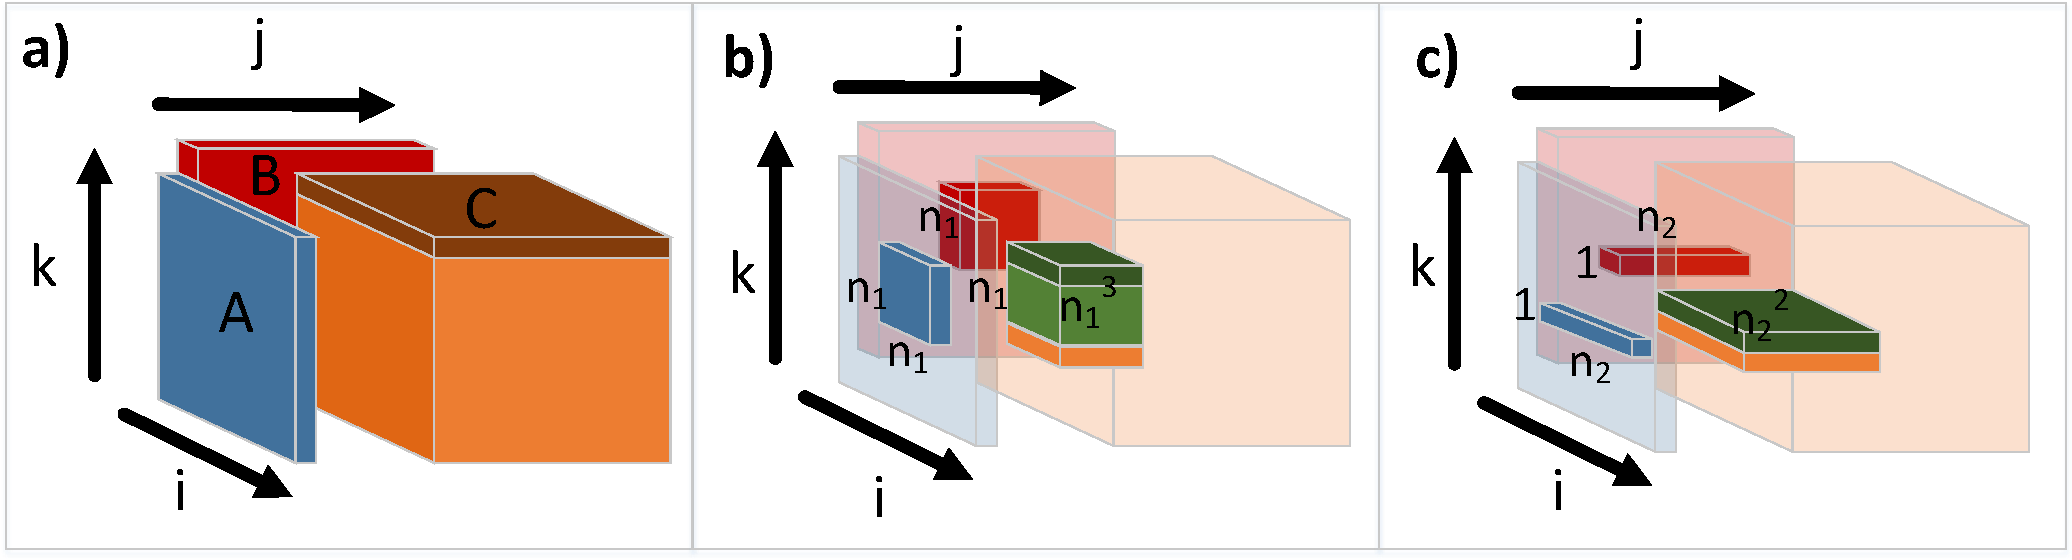
\includegraphics[width=\columnwidth]{figures/mmm_reuse}
%	%  \caption{MMM subset shape. a) 
%	%    geometric interpretation of $C = A B$ (orange cube represents 
%	%    3-dimensional iteration space of partial sums, matrix C is formed by 
%	%    reduction over dimension $k$ - represented by dark orange plane). b) 
%	%    optimal surface to volume subset shape. Note that in a subsequent 
%	%    subset computation only one of the three planes (blue, red or dark 
%	%    green) can be reused. c) the optimal subset shapes when 
%	%    data reuse is considered. In b) and c) blue, red, and orange surfaces 
%	%    form the dominator set, whereas dark green surface is the 
%	%    minimum set.}
%	%  \label{fig:mmmreuse}
%	%\end{figure}
%	
%	To show why Lemma 2 gives a tighter bound than Lemma 1, consider a CDAG of 
%	MMM.  We can draw it in a 3D iteration space $\mathcal{V}$.
%	(\cref{sec:iterationSpace}, ~\ref{fig:iterationSpace}). Then,
%	an $S$-partition is a decomposition of this space into subcomputations 
%	$V_i$ 
%	whose
%	number of inputs ($|\alpha_i| + |\beta_i| + |\gamma_i|$) is smaller than 
%	$S$.
%	When a subcomputation is viewed as a subspace in the iteration space $V_i 
%	\in 
%	\mathcal{V}$, this input constraint may be viewed as a generalization of 
%	the 
%	Loomis-Whitney inequality~\cite{loomisWhitney}, which relates a cardinality 
%	of 
%	a 
%	finite set in $\mathbb{Z}^t$ with cardinalities of its projections to all 
%	$t$ 
%	dimensions. This technique was used by Irony et al.~\cite{loomisApplied} to 
%	derive first parallel I/O MMM lower bounds.
%	
%	Assume that each subcomputation forms a cuboid $[a \times b \times c]$ in 
%	this
%	iteration space (we actually prove it in~\cref{sec:seqScheduling}). Its
%	faces form the dominator set.  Now based on Lemma~\ref{eq:redbluebound}, we 
%	construct a $2S$-partition with a
%	minimal cardinality, deriving subcomputations of a cubic ($a = b = c$) shape
%	(Figure~\ref{fig:iterationSpace} b), with a cube side $a = \sqrt{2S/3}$.  
%	Such
%	schedule will perform $2a^2 \frac{n^3}{a^3} =
%	\sqrt{\frac{3}{2}}\frac{2N^3}{\sqrt{S}}$ I/O operations. 
%	
%	Now, the question is: what is the size of a maximum reuse $R(S)$? Observe 
%	that
%	only one of three faces of this cuboid can be reused (used by a subsequent
%	subcomputation while still being in fast memory). This observation will 
%	help us
%	derive in (~\cref{sec:seqScheduling}) a "flat" shape (Figure 
%	\ref{fig:iterationSpace}
%	c) which performs $\frac{2N^3}{\sqrt{S}}$ I/O operations - an $\sqrt{3/2}$
%	improvement.
%	
%	
%	\section{\hspace{-0.5em}Optimal Sequential Matrix Multiplication}
%	\label{sec:seqOptimality}
%	
%	We now proceed to establish a tight sequential I/O lower bound of MMM. 
%	Using 
%	the 
%	mathematical machinery of 
%	Lemma~\ref{lma:reuse}, we show a constructive proof of $Q \ge 2MNK/\sqrt{S} 
%	+ 
%	MN$. This result has three main contributions (1) it is an additive 
%	improvement 
%	over the bound $2mnk/\sqrt{S} - 2S$ by Smith and van de 
%	Geijn~\cite{tightMMM} 
%	by an
%	additive factor of $2S + mn$, (2) the proof is constructive - what 
%	immediately 
%	follows is a corresponding schedule, (3) generality of a used technique is 
%	later used to derive I/O optimal parallel 
%	schedule~(\cref{sec:parOptimality}) 
%	and may be used in other 
%	linear algebra problems.
%	%
%	%\mac{the} I/O lower bound of MMM \mac{Now I'm confused, is it the
%	%new proof that is a new contribution, or the lower bound, or both? If the
%	%proof, then WHY does it matter that you have a new proof? What's the deep
%	%insight coming from this proof? And then why do you comment on tightening 
%	%the
%	%bound (below), if it's just a proof? And if it's the bound that is the new
%	%contribution, then say it (underline it better!) and remove the ``new'' 
%	%proof
%	%adjective. And if it's both, then just make this sound better here} 
%	%\mac{add
%	%here ``, namely''} $Q \ge \frac{mnk}{\sqrt{S}} + mn$ \mac{,} and show a
%	%schedule achieving it. This result will be used in
%	%Section~\cref{sec:parOptimality} to prove tight bounds for parallel 
%	%execution
%	%and a schedule that is \emph{independent of any combination of problem
%	%parameters} \mac{I would make this sentence the last in this paragraph}.
%	%%
%	%We derive \emph{all} constant terms improving the well-known asymptotic 
%	%results
%	%due to Hong and Kung~\cite{redblue} and Irony et al.~\cite{IronyMMM}, and
%	%tightening the bound $2mnk/\sqrt{S} - 2S$ by Smith and van de Geijn by an
%	%additive factor of $2S + mn$ \mac{I think it's better to place this 
%	%sentence
%	%right after the sentence with the lower bound, to immediately justify why 
%	%this
%	%new result matters}.
%	%
%	%\mac{Just in case, old beginning is below, commented}
%	%%   
%	%%   We now proceed to establish a key step to our main result. Using the 
%	%%   mathematical machinery of Lemma 2, we show a new proof of I/O lower 
%	%%bound 
%	%%of 
%	%%   MMM $Q \ge \frac{mnk}{\sqrt{S}} + mn$ and show a schedule achieving 
%	%%it. 
%	%%This 
%	%%   result will be used in Section~\cref{sec:parOptimality} to prove tight 
%	%%bounds 
%	%%   for parallel execution and a schedule 
%	%%   that is \emph{independent of any combination of problem parameters}.
%	%%   %
%	%%   We derive \emph{all} constant terms improving the well-known asymptotic
%	%%   results due to Hong and Kung~\cite{redblue} and Irony et 
%	%%al.~\cite{IronyMMM}, 
%	%%   and tightening the bound $2mnk/\sqrt{S} - 2S$ by Smith and van de 
%	%%Geijn by
%	%%   an additive factor of $2S + mn$.
%	%
%	%
%	%\greg{commented out the whole subsection Top-down vs bottom-up. It is 
%	%mentioned 
%	%in the intro and not needed here at all.}
%	
%	%\subsection{Top-Down vs Bottom-Up}
%	%
%	%\mac{The title is a bit confusing... Maybe we can remove it completely}
%	%
%	%\mac{No, I would start differently - with stating our approach, underlying 
%	%what
%	%is the paper contribution! E.g., "We do bottom-top (see Figure X), as 
%	%opposed 
%	%to [all
%	%others], [here is briefly why]}
%	%%
%	%Most of the current state-of-the-art algorithms, like 
%	%Cannon's~\cite{Cannon},
%	%SUMMA~\cite{summa}, 3D SUMMA~\cite{summa3d}, or the 2.5D scheme~\cite{25d}
%	%use the "top-down" approach, that is, aim for decomposing the global domain
%	%evenly into $p$ processes (Figure \ref{fig:topdown-vs-bottomup}).
%	%%
%	%To obtain our schedule and prove its optimality, we use "bottom-up" 
%	%approach,
%	%that is, defining the finest-granularity task for a single process and then
%	%identifying parallelization opportunities.  
%	%%
%	%\mac{Man, why do you provide this whole following part on task based
%	%programming?  What connection does it have? I would remove it completely, 
%	%or
%	%move to a place where task based stuff is used...} 
%	%%
%	%Intuitively, the "bottom-up" approach shares similarities with task-based
%	%programming~\cite{taskparalelism}, which has also be used in the context of
%	%linear algebra~\cite{taskMMM}. The difference, however, is in the
%	%\emph{granularity}: A task is a single, I/O optimal, rank-1 \mac{rank-1 
%	%was not
%	%defined} update (vector-vector outer product), instead of coarser grained
%	%rank-k \mac{rank-k was not defined} updates (matrix-matrix product) in
%	%recursive algorithms, like CARMA~\cite{CARMA}.
%	%%
%	
%	%
%	%\subsection{Tight MMM Lower Bound}
%	%\label{sec:seqScheduling}
%	%
%	%
%	%\greg{commented out the whole beginning}
%	%\mac{Bad, you should provide some beginning in this paragraph}
%	
%	%
%	%\mac{This title is too long}
%	%
%	%\mac{The following sequence is broken - how can algorithms
%	%derive their proofs? Moreover, ``derives'' should be ``derive'', right?}
%	%%
%	%"Top-down" algorithms, discussed in Section \ref{sec:seqOptimality}, 
%	%derives
%	%their 
%	%optimality proofs from maximizing computation to communication (input 
%	%volume) 
%	%ratio.
%	%%
%	%\mac{At this point, I again think that it's bad because you start with 
%	%describing
%	%others, and not the stuff in this paper}
%	%The key difference between them, as well as the original lower bound lemma 
%	%(inequality 
%	%\ref{eq:redbluebound}) and the lemma presented in this paper (inequality 
%	%\ref{eq:reusebound}) is the explicit notion of reuse. \mac{The following 
%	%sentence
%	%sounds like a reasonable first sentence in this section...} In this 
%	%section, 
%	%we prove 
%	%optimal sequential scheduling, \mac{The following sentence part is 
%	%broken?} 
%	%which later be used to derive parallelization 
%	%strategies.
%	%%
%	%\mac{Why do I care? Underline ``what'' parallelization strategies you will
%	%obtain - optimal? near-optimal? faster than others? Make this announcement 
%	%(parallelization strategies)
%	%sounds more interesting... Also, strategies of what?} 
%	%%
%	%The crucial insight is that it is independent of matrix dimensions 
%	%and machine model (distributed or shared memory).
%	%%
%	%\mac{What? At this point I'm confused. You always wrote about this stuff 
%	%being 
%	%independent of
%	%problem parameters. But saying it's independent of machine model is 
%	%extremely 
%	%confusing,
%	%considering the fact that you devoted so much space to describing I/O, etc 
%	%etc...}
%	%%
%	%\mac{In addition: ``it is independent of matrix dimensions
%	%and machine model'' is *not* a crucial insight... this is the advantage of
%	%this scheme. Insight is sth deep, some observation about the nature of 
%	%something.}
%	%%
%	%\mac{The following sentence: this is not a place for this... You should 
%	%discuss such
%	%things in related work. Sure, sometimes, one must discuss such connections 
%	%before
%	%related work, but make it concrete and to the point. Right now, you just 
%	%say 
%	%`` We do X differently than others''. Why do I care? How does it help me 
%	%understand
%	%this section better?}
%	%%
%	%We use different technique than used by Smith and van de Geijn, who proved 
%	%sequential lower bound $2mnk/\sqrt{S} - 2S$ and prove a lower bound 
%	%tighter 
%	%\mac{TIghter?
%	%Then why are we still better?} by 
%	%a constant factor of $2S$ :  $2mnk/\sqrt{S}$. Furthermore, the former 
%	%result 
%	%does not count storing the output, which yields additional $mn$ I/O 
%	%operations.
%	%\mac{Again, at this point I read 15 lines of text in this *core* and *key* 
%	%section
%	%that should focus on describing your idea, and still I have no idea... 
%	%more 
%	%than 30\%
%	%of this paragraph are some general notes, without obvious connection to 
%	%the 
%	%flow of
%	%*this* section, about others' work. How should it help the reader 
%	%understand 
%	%this
%	%section better?}
%	%
%	%\mac{The whole following part is again out of the place... I mean, 
%	%shouldn't 
%	%it be
%	%explained in Background? How does it relate to the models from Background?}
%	%We use the computation model from Hong and Kung~\cite{redblue}, that is:
%	%\begin{enumerate}
%	%  \item A machine has a fast memory of size $S$ and a slow memory of 
%	%infinite 
%	%  size,
%	%  \item all computations have to be performed inside fast memory, \mac{Huh?
%	%  But this sounds like you completely prevent *any* I/O during the 
%	%execution?
%	%  So what's the point of I/O complexity anyway?}
%	%  \item at the beginning of computation, all inputs are in slow memory, 
%	%and 
%	%  at the end of computation all the outputs must be stored back to slow 
%	%  memory. 
%	%\end{enumerate}
%	%
%	
%	\begin{thm}[Sequential Matrix Multiplication I/O lower bound] 
%		%Multiplying matrices of sizes $m \times k$ and $k \times m $ in the 
%		%computation 
%		%model from Definition~\ref{df:redbluegame} requires a minimum number 
%		%of 
%		%I/O 
%		%operations is $\frac{mnk}{\sqrt{S}} + mn$.
%		Multiplying matrices of sizes $m \times k$ and $k \times m $ requires a 
%		minimum 
%		number of $\frac{mnk}{\sqrt{S}} + mn$ I/O operations.
%		\label{thm:seqlowbounds}
%	\end{thm}
%	
%	\begin{proof}
%		
%		We first discuss a short intuition behind
%		the proof. Next, we provide all details.
%		
%		\macb{Proof Intuition}
%		%
%		Using Lemma~\ref{lma:reuse}, we first establish a valid subset $V_i$ of 
%		an
%		$S$-partition that achieves maximum computational intensity $\rho$ and 
%		find 
%		its
%		size (the number of vertices). Knowing $\rho$ and that there are $mnk$
%		vertices in the whole MMM CDAG, we find the total
%		I/O cost of the complete execution. Throughout the proof, in addition to
%		full details, we include intuitive interpretations of key steps. To
%		help keep up with the intuition, assume that $V_i$ is a 
%		cuboid~(\cref{sec:iterationSpace}), and that we want to find its 
%		optimal 
%		size 
%		under certain conditions.
%		
%		%\greg{your comments are commented out}
%		%  
%		%\mac{It may be a good idea to first have a titled paragraph like here, 
%		%with
%		%the outline of the proof, followed by the (titled again) rest.}
%		%%
%		%We first derive a size \mac{Did you define precisely ``size of an 
%		%S-partition?}
%		%and shape \mac{``shape of an S-partition'' was clearly not defined 
%		%before} 
%		%of
%		%an elementary \mac{What is ``elementary'' in this context? Again a 
%		%confusing
%		%word} S-partition subcomputation (subset) \mac{It seems these two words
%		%(subcomputation, subset) mean the same thing? Use only one
%		%consistently} $P$ that achieves 
%		%maximum computational intensity $\rho$ \mac{I would explain briefly 
%		%WHY 
%		%you 
%		%need
%		%to derive this particular S-partition}. We then show the 
%		%number of I/O operations per $P$ and derive the number of $P$ required 
%		%to 
%		%perform the whole computation. \mac{Again, I would briefly describe
%		%the general intuition of the whole proof and the most important steps}
%		
%		\macb{Full Proof}
%		%
%		In this proof, we will use the iteration space 
%		$\mathcal{V}$~(\cref{sec:iterationSpace}) to represent the 
%		CDAG of MMM.
%		By Definition~\ref{df:s-partition}, we divide the whole computation into
%		$H(S)$ subcomputations $V_i, i \in \{1,\dots H(S)\}$, such that 
%		$Dom(V_i), 
%		Min(V_i) \le 
%		S$. As stated in~(\cref{sec:iterationSpace}), the dominator set of 
%		$V_i$ is $Dom(V_i) =\phi_{ik}(V_i) \cup \phi_{kj}(V_i) \cup 
%		\phi_{ij}(V_i) 
%		= 
%		\alpha_i \cup \beta_i \cup \gamma_i$. Because all the read-after-write 
%		(RAW) 
%		dependencies are parallel to the vector~\textbf{k} (Line 5 in 
%		Listing~1), the projection of the minimum set $Min(V_i)$ onto the plane 
%		\textbf{ij} is also equal to $\gamma_i$ : ($\phi_{ij}(Min(V_i)) = 
%		\gamma_i$).
%		
%		\textbf{Intuition:}  $\alpha_i, \beta_i$ and
%		$\gamma_i$ are the faces of our cuboid $V_i$. The ``bottom'' face 
%		$\gamma_i$
%		(Figure~\ref{fig:iterationSpace}) is formed by partial results of $C$ 
%		from
%		previous subcomputations, and the ``top'' face is formed by partial 
%		results
%		evaluated by $V_i$, also forming input for
%		the next subcomputation. Because all the dependencies are facing 
%		``upwards'', 
%		the minimum set (the ``top'' face) is positioned directly above the 
%		required 
%		partial results of $C$, that is $\phi_{ij}(Dom(V_i)) = 
%		\phi_{ij}(Min(V_i))$.
%		
%		By the definition of $S$-partition, we have:
%		
%		\begin{gather}
%		\label{eq:dm}
%		|Dom(V_i)| = |\alpha_i| + |\beta_i| + |\gamma_i| \le S \\
%		\nonumber
%		|Min(V_i)| = |\gamma_i| \le S
%		\end{gather}
%		
%		
%		
%		On the other hand, the Loomis-Whitney
%		inequality~\cite{loomisWhitney} bounds the volume of $V_i$: 
%		
%		\begin{equation}
%		\label{eq:lm}
%		V_i \le \sqrt{|\alpha_i| |\beta_i| |\gamma_i|}
%		\end{equation}
%		
%		
%		%\textbf{Intuition:} Loomis-Whitney inequality bounds the volume of our 
%		%cuboid
%		%by the size of its faces.  \mac{I miss here some short text stating 
%		%this
%		%inequality and explaining how/why (formally) you can actually use it 
%		%in our
%		%context}
%		
%		Now we proceed to find the upper bound on the maximum reuse size $R(S) 
%		= 
%		\max_{j = 1 \dots
%			H(S)}(|V_{R,i}|)$. Consider two subsequent computations, $V_i$ and 
%		$V_{i+1}$.
%		Right after $V_i$, $\alpha_i$, $\beta_i$ and $\gamma_i$ may have red 
%		pebbles on 
%		them (they are in the fast memory). On the other hand the dominator set 
%		of 
%		$V_{i+1}$ is $Dom(V_{i+1}) = \alpha_{i+1} \sum \beta_{i+1} \sum 
%		\gamma_{i+1}$.
%		Then, the reuse set $V_{R,i+1}$ is an intersection of those two sets:
%		
%		\begin{gather}
%		\nonumber
%		V_{R,i+1}
%		\subset (\alpha_i \cup \beta_i \cup \gamma_i) \cap (\alpha_{i+1} 
%		\cup 
%		\beta_{i+1} \cup \gamma_{i+1}) \\
%		\label{eq:vri1}
%		= (\alpha_i \cap \alpha_{i+1}) \cup ( 
%		\beta_i \cap 
%		\beta_{i+1}) \cup (\gamma_i \cap \gamma_{i+1})
%		\end{gather}
%		
%		\textbf{Intuition:}
%		Visualizing $V_i$ and $V_{i+1}$ as two cuboids, they can only be 
%		positioned 
%		in 
%		the 3D space so that 
%		they share at most one of their sides (either $\alpha_i \cap 
%		\alpha_{i+1} 
%		\ne 
%		\emptyset$ or  $\beta_i \cap \beta_{i+1} \ne \emptyset$ or  $\gamma_i 
%		\cap 
%		\gamma_{i+1} \ne \emptyset$ ). If we allow other shapes than cuboids, 
%		their shared surface is a sum of its projections into the three 
%		planes,  
%		$\alpha_i \cap \alpha_{i+1}$,   $\beta_i \cap \beta_{i+1}$, and 
%		$\gamma_i 
%		\cap 
%		\gamma_{i+1}$.
%		
%		
%		Note that $\alpha_i, \beta_i \subset \mathcal{I}$ are inputs of the 
%		computation:
%		therefore,
%		by the Definition~\ref{df:redbluegame}, they start in the slow memory 
%		(they 
%		already have blue 
%		pebbles).
%		$\gamma_i$, on the other hand, is the projection of the
%		minimum set $\phi_{ij}(Min(V_i)) = \gamma_i$. Therefore, at the end of 
%		$V_i$, 
%		vertices in $Min(V_i)$ may have only red pebbles
%		placed on them (they may have not been stored back to the slow memory 
%		yet). 
%		Furthermore, by the Definition~\ref{df:s-partition}, these 
%		vertices have children that have not been pebbled yet. 
%		They either have to be reused forming the reuse set $V_{R,i+1}$, or
%		stored back, forming $W_{BR,i}$ and requiring the placement of the blue 
%		pebbles. 
%		Because by their definition, $\gamma_i \cap \alpha_i = \gamma_i \cap 
%		\beta_i = 
%		\emptyset$, we have $\gamma_i \cap V_{R,i+1} =  \gamma_i \cap
%		\gamma_{i+1}$ and $W_{BR,i} =  \gamma_i \setminus
%		\gamma_{i+1}$. Then, the number of I/O operations $Q_i$ performed by 
%		the 
%		subcomputation $V_i$ (cf. Lemma~\ref{lma:reuse}):
%		
%		\begin{equation}
%		\label{eq:qi}
%		Q_i \ge |Dom(V_i)| - |V_{R,i}| + |W_{BR,i}|
%		\end{equation} 
%		
%		\textbf{Intuition:} The dominator set of each subcomputation consists 
%		of 
%		certain
%		elements from input matrices $A$ and $B$, as well as the partial results
%		of $C$. The number of loads
%		required by $V_i$ is the size of the dominator set $Dom(V_i)$ reduced 
%		by the
%		elements already loaded (the reuse set $V_{R,i}$). The number of stores 
%		is 
%		equal to the
%		number of outputs $|\gamma_i|$  that are not reused in subcomputation 
%		$V_{i+1}$, that is, 
%		not contained in $|\gamma_{i+1}|$.
%		
%		We now proceed to find $\alpha_i, \beta_i$, and $\gamma_i$
%		that maximizes the computational
%		intensity $\rho_i = \rho$ (~\cref{sec:compIntensity}).
%		We can bound $\rho_i$ by inserting Equations~\ref{eq:dm}, \ref{eq:lm}, 
%		~\ref{eq:vri1} and~\ref{eq:qi}:
%		
%		\begin{gather}
%		\nonumber
%		\rho_i = \frac{|V_i|}{|Dom(V_i)| - |V_{R,i}| + |W_{BR,i}|} \\
%		\nonumber
%		\le 
%		\frac{\sqrt{|\alpha_i||\beta_i||\gamma_i|}}{|\alpha_i| + |\beta_i| + 
%			|\gamma_i| - |\gamma_i \cap \gamma_{i+1}| +  |\gamma_i \setminus 
%			\gamma_{i+1}|}
%		\end{gather}
%		
%		We immediately see that to maximize $\rho_i$, we have $\gamma_{i+1} = 
%		\gamma_i$, as it both maximizes $|\gamma_i \cap 
%		\gamma_{i+1}|$ and minimizes $|\gamma_i \setminus \gamma_{i+1}|$.
%		
%		We then formulate it as an 
%		optimization problem:
%		
%		%Inserting Equation~\ref{eq:vri1} to~\ref{eq:qi} we see that to 
%		%minimize 
%		%$Q_i$ 
%		%we have $\gamma_{i+1} = \gamma_i$, as it both maximizes $|\gamma_i 
%		%\cap 
%		%\gamma_{i+1}|$ and minimizes $|\gamma_i \setminus \gamma_{i+1}|$, 
%		%while 
%		%$|Dom(V_i)|$ does not depend on the choice of $\gamma_{i+1}$.
%		%
%		%
%		%W.l.o.g., assume that the subcomputation $V_i$ 
%		%achieves the maximum computational
%		%intensity $\rho_i = \rho$ (~\cref{sec:compIntensity}). To
%		%find $\alpha_i, \beta_i$ and $\gamma_i$, we formulate it as the 
%		%optimization 
%		%problem:
%		
%		
%		
%		%\begin{multline}
%		%\\
%		%\text{maximize } \rho = \frac{|V_i|}{|Dom(V_i)| - |V_{R,i}| + 
%		%|W_{BR,i}|} 
%		%\\
%		%\text{subject to: } |Dom(V_i)| \le S \\
%		%\end{multline}
%		
%		\begin{multline}
%		\\
%		\text{maximize }
%		\sqrt{\gamma_i}\frac{\sqrt{|\alpha_i| |\beta_i|}}{|\alpha_i| + 
%		|\beta_i|}\\
%		\text{subject to: } \\
%		|Dom(V_i)| = |\alpha_i| + |\beta_i| + |\gamma_i| \le S \\
%		|\alpha_i|, |\beta_i|, |\gamma_i| \in \mathcal{Z} 
%		\end{multline}
%		
%		Observe that to maximize $\frac{\sqrt{|\alpha_i| |\beta_i|}}{|\alpha_i| 
%		+
%			|\beta_i|}$ we have $|\alpha_i| = |\beta_i|$. Then the solution to 
%			this
%		maximization problem gives  $|\alpha_i| = |\beta_i| \rightarrow 0$, 
%		$|\gamma_i|
%		\rightarrow S$. But because $\alpha_i$, $\beta_i$ and $\gamma_i$ are 
%		sets 
%		of 
%		vertices, therefore $|\alpha_i|, |\beta_i|, |\gamma_i| \in \mathcal{Z}$.
%		Furthermore, we have $\phi_{kj}(\alpha_i) =
%		\phi_{ik}(\beta_i)$, $\phi_{ij}(\alpha_i) = \phi_{ik}(\gamma_i)$ and
%		$\phi_{ij}(\beta) = \phi_{kj}(\gamma)$. Finally, we get:
%		
%		\begin{multline}
%		\label{eq:seqSolution}
%		\\
%		|\alpha_i| = |\beta_i|= \left \lfloor{\sqrt{S + 1} - 1} \right \rfloor 
%		\\
%		|\phi_{kj}(\alpha)| = |\phi_{ik}(\beta)| = 1 \\
%		|\gamma| = |\alpha| |\beta| = \left \lfloor{(\sqrt{S + 1} - 1)^2} 
%		\right 
%		\rfloor 
%		\\
%		\end{multline}
%		
%		
%		
%		From now on, to keep the calculations simpler, we use the following 
%		approximation:
%		
%		\begin{equation}
%		\label{eq:approx}
%		\left \lfloor{\sqrt{S + 1} - 1} \right \rfloor \approx \sqrt{S}
%		\end{equation}
%		
%		All the following results may be easily rewritten using the precise 
%		formula 
%		and
%		are correct up to this approximation factor.
%		
%		Using the approximation~\ref{eq:approx}, we have $|V_i| = S, R(S) = 
%		V_{R,i} 
%		= 
%		|\gamma_i| = S, \rho =
%		\sqrt{S}/2$.
%		Finally,  by Corollary \ref{cor:q}:  
%		$$Q \ge
%		\frac{|V|}{\rho} = \frac{2mnk}{\sqrt{S}}$$ 
%		This is the I/O cost of putting a red pebble at least once on every 
%		vertex 
%		in 
%		$\mathcal{V}$. Note however, that we did not put any
%		blue pebbles on the outputs yet (all vertices in $\mathcal{V}$ had only 
%		red
%		pebbles placed on them during the execution). By
%		Definition~\ref{df:redbluegame}, we need to place blue pebbles on $mn$ 
%		output
%		vertices, corresponding to the output matrix $C$, resulting in 
%		additional 
%		$mn$
%		I/O operations, yielding final bound
%		$$Q \ge \frac{2mnk}{\sqrt{S}} + mn$$ 
%		%
%	\end{proof}
%	
%	\subsection{I/O Optimal Schedule}
%	\label{sec:seqScheduling2}
%	
%	The proof of Theorem~\ref{thm:seqlowbounds} is constructive:
%	that is, from it we immediately obtain a schedule achieving it. The optimal
%	subcomputation $V_i$ corresponds to $S$ calculated partial products of C. 
%	Its
%	inputs $\alpha$ and $\beta$ are subsets of a single column of $A$ and a 
%	single
%	row of $B$, both of length $\sqrt{S}$. This may be viewed as an outer 
%	product
%	formulation of MMM: each subcomputation is an outer product of two vectors 
%	of
%	length $\sqrt{S}$, with subsequent subcomputations updating this result
%	(Listing~\ref{lst:pseudocode}).
%	
%	\begin{lstlisting}[float=h, caption=Pseudocode of I/O optimal sequential 
%	MMM, 
%	label=lst:pseudocode]
%	T = $\sqrt{S}$
%	for i_1 = 1:m/T
%	for j_1 = 1:n/T
%	for r = 1:k    % k is the outer loop
%	%elementary subcomputation V
%	for i_2 = i_1*T : (i_1+1)*T
%	for j_2 = j_1*T : (j_1+1)*T
%	C(i_2,j_2) = C(i_2,j_2) + A(i_2,r)*B(r,j_2)
%	end for
%	end for 
%	end for
%	end for 
%	end for
%	\end{lstlisting}
%	%
%	%We note that an implementation based on this outer
%	%schedule is the Goto algorithm~\cite{Goto}. 
%	
%	%-------------old version starts here----------%
%	%\greg{------------old version starts here -----------} 
%	%
%	%
%	%
%	%Let's \mac{Let's is too informal} represent the matrix multiplication 
%	%operations \mac{What are ``matrix multiplication operations''?
%	%again, confusing. Intuitively it may be clear, but this must be precise. 
%	%The 
%	%actual products of matrix elements? the sums? more precision} as the three 
%	%dimensional 
%	%iteration space \mac{This is much more your domain and not main, but 
%	%``iteration space'' also
%	%sounds quite vague}. Let $i,j,k$ be dimensions corresponding to matrix 
%	%sizes 
%	%$m,n,k$, that is, matrix $A$ lays on the plane $ik$, matrix $B$ lays on 
%	%the 
%	%plane $kj$ and matrix $C$ lays on the plane $ij$ \mac{This again is 
%	%somewhat 
%	%confusing. What is ``plane'' mathematically here?
%	%This is proof, all must be clear. Define plane... But then I know, there 
%	%are 
%	%many
%	%of these concepts (as we discussed while hiking), and defining them all
%	%would be very tedious... My recommendation - \ul{I suggest you read several
%	%proofs from top math conferences related to this type of things, and see 
%	%how 
%	%people deal with this}}.
%	%
%	%\mac{\ul{Another important comment:} at this point, it becomes clear that
%	%the paper lacks some background into the MM stuff. I mean, you need to
%	%lay out the setting... All these MM-related concepts such as laying 
%	%matrices
%	%A, B, C onto different ``planes of computation'' must be introduced in
%	%Background.}
%	%%
%	%Assume that the searched subset \mac{I would use some symbol for this 
%	%subset
%	%that maximizes intensity} computes $\mathcal{V}$ partial products $c = c + 
%	%ab$
%	%\mac{what? why $c = c + ab$? Mathematically, unless $ab=0$, it's never 
%	%true,
%	%right?} of $C$ \mac{\ul{First comment:} Also, it's confusing: what are
%	%``products of $C$''??}. Then, the projection of $\phi_{ik}(\mathcal{V})$
%	%\mac{``Projection'' was never defined (extremely confusing). \ul{Second
%	%comment:} Moreover: what is this $\mathcal{V}$? it is also not defined. In 
%	%the
%	%sentence before, it sounds like a number (``$\mathcal{V}$ products''), but 
%	%here
%	%it sounds more like something more complex than a number? Again confusing.
%	%\ul{Third comment}: is it "the projection of" OR "the projection"? It 
%	%makes a
%	%huge difference. Now it sounds like it should be "the projection" (and is
%	%wrongly "the projection of"} onto plane $ik$ correspond 
%	%\mac{``corresponds''
%	%instead of ``correspond''?} to the required inputs from $A$.  \mac{Very
%	%confusing - WHY does this projection correspond to the input? It will be
%	%unclear to the reader... Maybe with the proper background it will clarify?}
%	%Let's \mac{Let's is informal - better just "Denote"} denote $A$'s input
%	%$\phi_{ik}(\mathcal{V}) = \alpha$ \mac{Symbol for denote should be 
%	%different
%	%from $=$, I would just use a word ``as''}.  Similarly, 
%	%$\phi_{kj}(\mathcal{V})
%	%= \beta$ and $\phi_{ij}(\mathcal{V}) = \gamma$, which correspond to partial
%	%results of $C$ being updated \mac{This part of sentence is again extremely
%	%confusing. What partial results? Why? You just wrote about some inputs, why
%	%suddenly something corresponds to some partial results of $C$?  and what 
%	%does
%	%it mean ``$C$ being updated''? How updated?}. Furthermore, note that 
%	%$\gamma$
%	%is also the output of the subcomputation \mac{what ``subcomputation''?  In 
%	%the
%	%context of S-partitions? Or is it something purely MM-related?  If yes, 
%	%what
%	%exactly? Adding one element to one element of $C$? computing a block of 
%	%$C$?
%	%what?}, as those inputs are updated \mac{How updated? Confusing again...}.
%	%
%	%To compute $\mathcal{V}$ partial products $c = c + ab$ of $C$ \mac{Same
%	%comments as before, it's confusing on that these symbols really mean. \ul{I
%	%mean, the point is that to someone who is specializing in MM stuff, this 
%	%will
%	%more or less be somewhat clear}: c = c + ab will mean that you update some
%	%element of C with corresponding ab. However, ANY OTHER person will be lost
%	%after the FIRST SENTENCE of this section / proof. In addition, even if a
%	%reviewer related to MM understands the stuff, it will not help in 
%	%persuading
%	%him/her to accept the paper, because they will notice all these confusing
%	%parts}, we need $\alpha$ and $\beta$ elements of matrices $A$ and $B$
%	%\mac{What are precisely these elements of matrices?} and $\gamma$ elements 
%	%of
%	%$C$, corresponding to the updated values of $c$ (Figure \ref{fig:mmmreuse})
%	%\mac{This sentence before is also confusing with respect}.  Therefore, the
%	%input size \mac{What is ``input'' in this current context?} (surface in
%	%geometric interpretation \mac{You never defined anything related to the
%	%geometric interpretation}) is $\mathcal{I} = |\alpha| + |\beta| + |\gamma|$
%	%\mac{This equality is unclear - not obvious why it should be true}. 
%	%According
%	%to the definition of S-partition, $$\mathcal{I} = |\alpha| + |\beta| +
%	%|\gamma|\le S$$ \mac{This previous inequality is important - it combines 
%	%MM and
%	%I/O complexity...  But it's also unclear why this is the case. This must be
%	%explained more extensively / appropriately}.  From Loomis-Whitney 
%	%inequality
%	%\cite{loomisWhitney}, we have the upper bound on $$\mathcal{V} \le
%	%\sqrt{|\alpha| |\beta| |\gamma|}$$ \mac{I would consider putting 1-2 
%	%sentences
%	%on the Loomis-Whitney stuff... maybe}.  The upper bound on te \mac{the?} 
%	%reuse
%	%$R(S)$ \mac{At this point, no idea what R(S) is. It was defined, but it 
%	%gets so
%	%complex at this stage that readers won't know. I suggest to remind somehow 
%	%what
%	%it is, intuitively. \ul{Another suggestion: MAYBE a solution to the whole
%	%problem of the complexity is to, like I guess we already discussed, is to 
%	%start
%	%early in background with matrix multiplication, and then, at every step of 
%	%the
%	%I/O stuff, provide relations to MM. THis way, people will always get these 
%	%two
%	%next to each other in their minds}} is a largest \mac{The largest?} 
%	%projection
%	%of $\mathcal{V}$ to any surface $\mathcal{P}$ in the $ijk$ space \mac{To an
%	%arbitrary one? Or to one of the 3 ``canonical'' ones?}: $$R(S) \le
%	%\max_\mathcal{P}(|\phi_\mathcal{P}(V)|)$$ \mac{What is the definition of 
%	%the $|
%	%\cdot |$ symbol above in the current context?} Furthermore $\alpha$ and 
%	%$\beta$
%	%are the inputs and do not need to be stored \mac{Really? Why not? AN 
%	%average
%	%reader will think it's not true, because you always must store input 
%	%somewhere?
%	%Make it precise what it means (no I/O)?}.  $\gamma$, on the other hand, is 
%	%the
%	%set of partial results and either has to be reused or stored, increasing 
%	%the
%	%I/O cost \mac{What is precisely ``I/O cost''? I know, I know, that's all 
%	%what
%	%the paper is about, but I think it might not hurt to clearly state / 
%	%define at
%	%the very beginning some cost function for this thing...}. 
%	%
%	%Let's \mac{Informal} denote $\alpha_i$ and $\beta_i$ as inputs of $i$-th
%	%subcomputation \mac{What is ith subcomputation? How does it relate to the 
%	%I/O
%	%business? Confusing, not clear}, $\gamma_i$ as its input and output, and 
%	%$R_i$
%	%as its reuse (subset of inputs that is already in the fast memory \mac{Why 
%	%do
%	%you suddenly remind HERE what reuse is, and did not do this several lines
%	%above?}). Then, $$R_i = (\alpha_i \cap \alpha_{i-1}) \cup (\beta_i \cap
%	%\beta_{i-1}) \cup (\gamma_i \cap \gamma_{i-1}) $$ \mac{This series of 
%	%unions is
%	%unclear} Note that $|\gamma_i \setminus \gamma_{i+1}|$ outputs have to be
%	%stored back to the memory \mac{why?}. The I/O cost of $i$-th 
%	%subcomputation is
%	%$$Q_i = |\mathcal{I}| - |R_i| + |\gamma_i \setminus \gamma_{i+1}|$$.
%	%
%	%The projection plane $\mathcal{P}$ \mac{What is ``projection plane''?}
%	%minimizing $Q_i$ \mac{What does it mean ``minimizing'' in the current 
%	%context?
%	%meaning, it's not fully clear what the connection between planes and
%	%minimization is} is therefore $\mathcal{P} = ij$, resulting in $\gamma_i =
%	%\gamma_{i+1}$\mac{What does this last equality intuitively mean?}. 
%	%Intuitively,
%	%this is clear that we should reuse partial results of $C$ immediately, 
%	%instead
%	%of storing them back to the memory. Therefore, to obtain the optimal
%	%subcomputation, we formulate it as the optimization problem 
%	%\mac{``Therefore''
%	%- it is not clear why ``formulating it as an optimization problem'' is a
%	%logical consequence of the previous sentence}:
%	%
%	%\begin{multline}
%	%\\
%	%\text{maximize } \rho = \frac{|\mathcal{V}|}{\mathcal{I} - |R|} \le 
%	%\frac{\sqrt{|\alpha| |\beta| |\gamma|}}{|\alpha| + |\beta|}\\
%	%\text{subject to: } |\alpha| + |\beta| + |\gamma| \le S \\
%	%\end{multline}
%	%
%	%Exploiting the symmetry of the domain \mac{What is ``the symmetry of the
%	%domain''?} by plane \mac{What does it mean ``by plane'' in this context?}
%	%\textbf{(i + j)k} \mac{Why bold now and not before?}, we have  $|\alpha| =
%	%|\beta|$. Now the solution to this problem gives $|\alpha| = |\beta|
%	%\rightarrow 0$, $|\gamma| \rightarrow S$ \mac{Unclear how you get these
%	%results}.  Restricting the solution to the integer lattice ($\alpha, \beta,
%	%\gamma \in \mathbb{Z}$) we get the optimal shape of the subcomputation
%	%\mac{Again, this shape of subcomputation should be more clear}:
%	%
%	%\begin{multline}
%	%%\label{eq:seqSolution}
%	%\\
%	%|\phi_{ij}(\alpha)| = |\phi_{ik}(\alpha)|  = |\phi_{ij}(\beta)| = 
%	%|\phi_{kj}(\beta)|= \sqrt{S + 1} - 1 \\
%	%|\phi_{kj}(\alpha)| = |\phi_{ik}(\beta)| = 1 \\
%	%|\gamma| = |\alpha| |\beta| = (\sqrt{S + 1} - 1)^2 \\
%	%\end{multline}
%	%
%	%This corresponds to a single column of $A$ and row of $B$ of length 
%	%$\sqrt{S +
%	%1} - 1$ and a square subset of $C$ of $(\sqrt{S + 1} - 1)^2$.  
%	%\textbf{From now
%	%on, to keep the notation \mac{It's not notation that you keep simpler here,
%	%it's calculations?} simpler, we approximate} 
%	%\begin{equation}
%	%\label{eq:approx}
%	%\sqrt{S + 1} - 1 \approx \sqrt{S}
%	%\end{equation}
%	%All the following results may be easily rewritten using the precise 
%	%formula and
%	%are correct up to this approximation factor.
%	%
%	%
%	%This result immediately gives $\mathcal{V} = S, R(S) = S, \rho = 
%	%\sqrt{S}/2$
%	%\mac{How do you get these? Completely unclear} and finally, according to
%	%corollary \ref{cor:q}:  $Q \ge \frac{|V|}{\rho} = \frac{2mnk}{\sqrt{S}}$. 
%	%This
%	%is only the input cost \mac{Huh? What is the input cost? Why input cost?}, 
%	%as
%	%for now, we assumed that all the outputs were reused. However, $mn$ outputs
%	%  have to be stored back to the memory, yielding additional $mn$ I/O 
%	%operations
%	%  \mac{Unclear sentence}. 
%	%
%	%%-------------old version ends here----------%
%	%\greg{------------old version ends here -----------} 
%	
%	\bibliographystyle{ACM-Reference-Format}
%	\bibliography{mmm-ppopp}
%	
%	
%	
%\end{document}











%%%%%%%%%%%%%%%%%%%%%%%%%%%%%%%%
%-------------- version with R(S) and T(S) starts here ----------
%%%%%%%%%%%%%%%%%%%%%%%%%%%%%%%%





%% For double-blind review submission, w/o CCS and ACM Reference (max 
%%submission space)
\documentclass[sigplan,review,anonymous,10pt]{acmart}\settopmatter{printfolios=true,printccs=false,printacmref=false}
%% For double-blind review submission, w/ CCS and ACM Reference
%\documentclass[sigplan,review,anonymous]{acmart}\settopmatter{printfolios=true}
%% For single-blind review submission, w/o CCS and ACM Reference (max 
%%submission space)
%\documentclass[sigplan,review]{acmart}\settopmatter{printfolios=true,printccs=false,printacmref=false}
%% For single-blind review submission, w/ CCS and ACM Reference
%\documentclass[sigplan,review]{acmart}\settopmatter{printfolios=true}
%% For final camera-ready submission, w/ required CCS and ACM Reference
%\documentclass[sigplan]{acmart}\settopmatter{}

\usepackage{soul}

\usepackage{color, colortbl}

%\usepackage{booktabs} % For formal tables
%\documentclass{article}
%\usepackage{floatrow}
\usepackage{rotating}
\usepackage{graphicx}
\usepackage{multirow}
%\usepackage[dvipsnames]{xcolor}
\usepackage{amsfonts}
\usepackage{amsmath}
\usepackage{amssymb}
\usepackage{mathtools}
\usepackage{wrapfig}
\usepackage{listings}
\usepackage{graphicx}
\usepackage{caption}
\usepackage{tabularx}
%\usepackage{amsthm}
%\usepackage[section]{placeins}
\usepackage{enumitem}
%\usepackage[a4paper, total={7in, 10.5in}]{geometry}
\usepackage[font={small}]{caption}
%\usepackage[font={bf,sf,small}]{caption}
%\usepackage[linesnumbered,ruled]{algorithm2e}
\usepackage{algpseudocode}
\captionsetup{labelfont=bf,textfont=bf}
\usepackage[font={bf,sf,scriptsize}]{subfig} 
\usepackage{amsthm}

%
%\usepackage[utf8]{inputenc}
%\usepackage{url}
%\usepackage{amsmath,amsthm,amssymb,amsfonts}
\usepackage{algorithm}
\usepackage{algpseudocode}
\usepackage{algorithmicx}
%\usepackage{graphicx}
%\usepackage{caption}
%\usepackage[thinlines]{easytable}
%\usepackage{pdfpages}
%\usepackage{fancyhdr}
%\usepackage{booktabs}
%\usepackage{footnote}
%\usepackage{footmisc}
%\usepackage{mathtools}
%\usepackage{multirow}
%%\usepackage{siunitx}
%%\usepackage{booktabs}
%%\usepackage{blindtext}
%%\usepackage[pdfencoding=auto,psdextra]{hyperref}
%
%\fancyhf{}
%\renewcommand{\headrulewidth}{0pt}
%\renewcommand{\footrulewidth}{0pt}
%
%\DeclarePairedDelimiter\abs{\lvert}{\rvert}
%
%\makeatletter
%\let\oldabs\abs
%\def\abs{\@ifstar{\oldabs}{\oldabs*}}
%\makeatother
%\def\E{\mathbb{E}}
%
%\makeatletter
%\g@addto@macro \normalsize {%
%	\setlength\abovedisplayskip{5pt plus 2pt minus 2pt}%
%	\setlength\belowdisplayskip{5pt plus 2pt minus 2pt}%
%}
%\makeatother


\renewcommand{\algorithmicrequire}{\textbf{Input:}}
\renewcommand{\algorithmicensure}{\textbf{Output:}}

\newcommand\numberthis{\addtocounter{equation}{1}\tag{\theequation}}
\def\NoNumber#1{{\def\alglinenumber##1{}\State #1}\addtocounter{ALG@line}{-1}}



%\usepackage[demo]{graphicx}
%\setlength{\footskip}{15pt}
%\usepackage[utf8]{inputenc}
%\usepackage[english]{babel}
\newtheorem{theorem}{Theorem}[section]
\newtheorem*{corollary*}{Corollary}
\newtheorem{corollary}{Corollary}[theorem]
%\newtheorem{lemma}[theorem]{Lemma}
\newcommand\todo[1]{\textcolor{red}{#1}}
\newcommand\greg[1]{\textcolor{blue}{[Greg: #1]}}
\newcommand\toskip[1]{\textcolor{green}{[possibly to skip: #1]}}
\newcommand\mac[1]{\textcolor{red}{[Mac: #1]}}

\newcommand*\diff{\mathop{}\!\mathrm{d}}
\newcommand*\Diff[1]{\mathop{}\!\mathrm{d^#1}}

\DeclareMathOperator*{\argmax}{arg\,max}
\DeclareMathOperator*{\argmin}{arg\,min}

%  \lstset{language=C,
%    keepspaces=true,
%    frame=tb,
%    basicstyle=\ttfamily,
%    columns=fixed,
%    morekeywords={enddo},
%    mathescape}

\definecolor{darkgrey}{RGB}{70,70,70}
\definecolor{lightgrey}{RGB}{200,200,200}

\lstset{language=C,
        escapechar=|,
        keepspaces=false,
        frame=tb,
        framexleftmargin=1.5em,
        basicstyle=\tt\scriptsize,
        columns=fixed,
        %otherkeywords={enddo,forall,bool,true,false, int64_t, MPI_Op, in, 
        %parallel, function},
        otherkeywords={enddo,end,forall,bool,true,false, int64_t, MPI_Op, 
        function},
        tabsize=2,
        breaklines=true,
        captionpos=b,
        %aboveskip=-1.5em,
        %belowskip=-0.5em,
        numbers=left,
        xleftmargin=1.5em,
        keywordstyle=\bfseries\color{black!400!black},
        stringstyle=\color{orange},
        commentstyle=\color{darkgrey},
        numberstyle=\scriptsize,numbersep=3pt,mathescape}


\usepackage[font={bf,sf,scriptsize}]{caption}
%\usepackage[font={bf,sf,scriptsize}]{subfig}

\usepackage{cleveref}
\usepackage[utf8]{inputenc}
\crefname{section}{§}{§§}
\Crefname{section}{§}{§§}

\newtheorem{defn}{Definition}
\newtheorem{thm}{Theorem}
\newtheorem{clm}{Claim}
\newtheorem{crl}{Corollary}
\newtheorem{lma}{Lemma}
%\newtheorem{proof}{Proof}
%\newtheorem*{proof*}{Proof}
\newtheorem{observation}{Observation}

\newcommand{\macb}[1]{\textbf{\textsf{#1}}}

\DeclareSymbolFont{matha}{OML}{txmi}{m}{it}% txfonts
\DeclareMathSymbol{\varS}{\mathord}{matha}{83}

\acmConference[PPoPP'19]{ACM SIGPLAN Annual Symposium on Principles and 
Practice of Parallel Programming}{February 16--20, 2019}{Washington DC, USA}
% \acmYear{}
% \acmISBN{} 
% \acmDOI{}
\startPage{1}

%% Copyright information
%% Supplied to authors (based on authors' rights management selection;
%% see authors.acm.org) by publisher for camera-ready submission;
%% use 'none' for review submission.
\setcopyright{none}
%\setcopyright{acmcopyright}
%\setcopyright{acmlicensed}
%\setcopyright{rightsretained}
%\copyrightyear{2018}           %% If different from \acmYear

%% Some recommended packages.
\usepackage{booktabs} 
\usepackage{makecell}
\hypersetup{draft}

\usepackage{pifont}

\begin{document}

%% Title information

\title[I/O-Optimal Dimensionless Matrix Multiplication]{\vspace{-1em}Breaking 
The 
Monopoly of Dimensions: Towards I/O-Optimal Matrix Multiplication}


\author{First1 Last1}
\authornote{with author1 note}          %% \authornote is optional;
                                        %% can be repeated if necessary
\orcid{nnnn-nnnn-nnnn-nnnn}             %% \orcid is optional
\affiliation{
  \position{Position1}
  \department{Department1}              %% \department is recommended
  \institution{Institution1}            %% \institution is required
  \streetaddress{Street1 Address1}
  \city{City1}
  \state{State1}
  \postcode{Post-Code1}
  \country{Country1}                    %% \country is recommended
}
\email{first1.last1@inst1.edu}          %% \email is recommended

%% Author with two affiliations and emails.
\author{First2 Last2}
\authornote{with author2 note}          %% \authornote is optional;
                                        %% can be repeated if necessary
\orcid{nnnn-nnnn-nnnn-nnnn}             %% \orcid is optional
\affiliation{
  \position{Position2a}
  \department{Department2a}             %% \department is recommended
  \institution{Institution2a}           %% \institution is required
  \streetaddress{Street2a Address2a}
  \city{City2a}
  \state{State2a}
  \postcode{Post-Code2a}
  \country{Country2a}                   %% \country is recommended
}
\email{first2.last2@inst2a.com}         %% \email is recommended
\affiliation{
  \position{Position2b}
  \department{Department2b}             %% \department is recommended
  \institution{Institution2b}           %% \institution is required
  \streetaddress{Street3b Address2b}
  \city{City2b}
  \state{State2b}
  \postcode{Post-Code2b}
  \country{Country2b}                   %% \country is recommended
}
\email{first2.last2@inst2b.org}         %% \email is recommended



\appendix


\section{I/O Lower Bounds for Arbitrary CDAGs}
\label{sec:introIO}
In this section we shortly introduce a general mathematical machinery we use 
to 
proof 
the I/O optimality of COMM. We extend Lemma~\ref{lma:spartlemma} by 
Hong and 
Kung~\cite{redblue}, which provides a method to find an I/O lower bound for a 
given CDAG. This lemma, however, does not give a tight bound, as it 
overestimates a \emph{reuse set} size (cf. 
Lemma~\ref{lma:reuse}). Our key result here, Lemma~\ref{lma:reuse} 
allows us to derive a constructive proof of a tighter I/O lower bound for a 
sequential execution of MMM CDAG~(\cref{sec:seqOptimality}). We use this 
result 
in~(\cref{sec:parOptimality}) to prove the parallel I/O optimality of COMM.

Our method heavily relies on a red-blue pebble game 
(Definition~\ref{df:redbluegame}) 
and an $S$-partition abstractions (Definition~\ref{df:s-partition}) introduced 
by Hong and Kung.

\subsection{Red-Blue Pebble Game}
A red-blue pebble game is an abstraction modeling an execution of an algorithm 
in a two-level memory structure with a 
small-and-fast
as well as large-and-slow memory. A red (or a blue) pebble placed on a vertex 
of a CDAG denotes that this data is inside a fast (or slow) memory.  It is a 
powerful tool, extensible to
arbitrarily many memory levels~\cite{redblueHierarchy}, that was used to derive
lower bounds for algorithms such as sorting or FFT~\cite{redblue}. 

\macb{Intuition}
%
In the red-blue pebble game, a red (or blue) pebble placed on a vertex denotes 
that its value is inside the fast (or slow) memory.
%
%A computation of a 
%CDAG starts with placing
%certain \emph{pebbles} on its input vertices\greg{changed "certain 
%number of pebbles" to "certain pebbles". The first one was just wrong.}, 
%which 
%corresponds to 
%loading the
%data from the slow to the fast memory. 
%
The actual computation (referred to as
\emph{pebbling}) is a series of allowed moves (e.g., moving a pebble from one
vertex to another) that correspond to load, store, compute, or
freeing-memory operations.
%
The \emph{I/O cost of a computation} is the number of pebble moves that
correspond to loads and stores between the slow and the fast memory; finding 
the pebbling that minimizes
this cost is PSPACE-complete~\cite{redbluecomplete, pebblegameregister}. 

\begin{defn}[Red-Blue Pebble Game~\cite{redblue}] \label{df:redbluegame}
	Let $G = (V,E)$ be a CDAG. 
	In the initial/terminal configuration, only inputs/outputs of the CDAG have
	blue pebbles.
	%
	There can be at most $S$ red pebbles used. A complete CDAG computation is a
	sequence of moves that lead from the initial to the terminal pebble
	configuration.
	%
	The allowed moves are as follows: \ding{172} placing a red pebble on any 
	vertex
	with a blue pebble (load), \ding{173} placing a blue pebble on any vertex 
	with 
	a red
	pebble (store), \ding{174} placing a red pebble on a vertex whose parents 
	have 
	all red
	pebbles (compute), \ding{175} removing any pebble (red or blue) from any 
	vertex 
	(freeing memory).
\end{defn}

An I/O optimal execution of a CDAG corresponds to a sequence of moves (called 
\emph{pebbling} of a graph) which minimizes load \ding{172} and store 
\ding{173} moves.

\macb{Connections to MMM}
%
For a CDAG of MMM, an example pebbling moves include placing red pebbles on 
some vertices
corresponding to elements of matrices $A$ and $B$ (load operations), placing 
red
pebbles on the corresponding elements of $C$ (compute), removing red
pebbles from the loaded inputs (freeing memory) and placing blue pebbles on the
computed elements of $C$ (store). 

\subsection{$S$-Partitions}


The notion of an \emph{$S$-partition} facilitates deriving lower bounds on the
I/O computation cost~\cite{redblue}. Here, one divides a given CDAG into
consecutive \emph{subcomputations}, each of which requires at least $S$ load 
and store
operations. The key element in more straightforward
lower bound proofs is to analytically bound the size (vertex count) of
the largest subcomputation, given its input and output size (i.e., the number
of vertices outside (inside) the subcomputation that have a child inside
(outside) of it). 
%
%\macb{Intuition}
%
%Intuitively, the $S$-partition technique may be seen as a generalization of
%the Loomis-Whitney inequality~\cite{loomisWhitney}, which is used in linear
%algebra for bounding the amount of I/O~\cite{loomisApplied}: both techniques
%aim at finding the optimal surface (communication) to volume (computation)
%ratio in a given setting. 
%
%$S$-partition was used to derive the first I/O bounds for matrix
%multiplication, FFT, or odd-even transposition sorting~\cite{redblue}.
%
%\macb{Details}
%
Formally:

\begin{defn}[$S$-partition of a CDAG~\cite{redblue}] \label{df:s-partition}
	%
	Let $G = (V,E)$ be a CDAG. An $S$-partition of $G$ is a collection $\{V_1, 
	...,
	V_h\}$ of $h$ subcomputations of $ V$ such that: \ding{192} $V_i \cap V_j
	=\emptyset\ $ and $\bigcup_{i=1}^{h} V_i=V$ for any $1 \le i,j \le h$,
	\ding{193} $\forall i\quad |Dom(V_i)| \le S$, \ding{194} $\forall i\quad
	|Min(V_i)| \le S$, and \ding{195} there is no cyclic dependence between
	subcomputations.
	%   
	% \begin{itemize} \item $\forall_{1 \le i,j \le h}\quad V_i \cap V_j
	% =\emptyset\ $ and $\ \bigcup_{i=1}^{h} V_i=V$ \item $\forall i\quad
	% |Dom(V_i)| \le S$ \item $\forall i\quad |Min(V_i)| \le S$ \item there is 
	%no
	% cyclic dependence between subcomputations.  \end{itemize}
	%
\end{defn}

$Dom(V_i) \not \subset V_i$ is the \emph{dominator set}: a set of vertices 
such 
that
every path from an input of the CDAG to a vertex in $V_i$ contains some 
vertex in in
$Dom(V_i)$.
%
$Min(V_i) \subset V_i$ is the \emph{minimum set} of $V_i$: it contains vertices
that do not have any children in $V_i$. 
%
%Throughout this paper, we will use \emph{subset} and \emph{subcomputation}
%interchangeably, to emphasize its interpretation in the context of 
%scheduling. 
%
Finally, $H(S)$ is the cardinality of the smallest valid $S$-partition of a
given CDAG.

We use a symbol $\mathcal{S}(S) = \{V_1, \dots , V_h\}$ to 
denote an $S$-partition. 
%
% there is a
%lower bound on the cardinality of a valid $S$-partition.  We denote this
%minimal number of vertex sets with a dedicated symbol $H(S)$.

\macb{Connections to MMM}
%
In MMM, a subcomputation $V_i$ is a calculation of partial sums of $C$ that can
be computed with at most $S$ elements of $A$ and $B$, and that contributes to
at most $S$ outputs. Those elements from $A$ and $B$, as well as previous
values of $C$ being updated, form $Dom(V_i)$. Then, $Min(V_i)$ corresponds to
the result of this subcomputation (cf.~
Figure~\ref{fig:iterationSpace}). $H(S)$ denotes 
the
number of such subsets required to calculate the final result. Assuming that 
each subcomputation computes the same number of partial results 
$\forall_{i,j}|V_i| = |V_j|$, and observing the total number of partial 
results 
$|V| = mnk$, we have $H(S) = \frac{mnk}{V_i}$.
% (geometrically
%\mac{what does geometrically mean?}, \mac{the} number of subsets require
%\mac{required} to fill the entire 3D iteration space \mac{what 3D space? was
%*never* defined or even mentioned... Already complained. I think the best 
%place
%is the background subsection dedicated to MMM. It can be very brief (1-2 
%sentences)}).

\subsection{Existing General I/O Lower Bound}
\label{sec:spartProof}

%\greg{Observation: 2S-partition reduces scheduling problem (P-space) 
%to 
%partitioning problem (NP-complete)?}
%\greg{...... UPDATE: I don't show here the proof of NP-completeness 
%of 
%S-partitioning. Too much space. Better skip this observation}

We now cite a \emph{general} lower bound on the cost of \emph{any} I/O
computation~\cite{redblue} and sketch the proof, which is the basis for our
\emph{tighter general} bound on the I/O cost (Lemma~\ref{lma:reuse}).

\macb{Intuition}
%
The key notion in the existing bound is to use $2S$-partitions for a given fast
memory size~$S$.
%
For some subcomputation $V_i$, if $|Dom(V_i)| = 2S$ vertices, then at most $S$
of them could contain a red pebble before $V_i$ begins.  Thus, at least $S$
additional pebbles need to be loaded from the memory.  The similar argument
goes for $Min(V_i)$. Therefore, knowing the lower bound on the number of sets
$V_i$ in a valid \emph{$2S$-partition}, together with the observation that each
$V_i$ performs at least $S$ I/O operations, we have:
%
%  a \emph{$2S$-partitioning} of the
%graph. Thus, each subcomputation $V_i$ requires $2S$ input elements (the
%dominator set) to perform the computation. Because at most $S$ elements could
%already be in the fast memory from the previous computation (recall that the
%size of the fast memory is $S$), the remaining $S$ elements have to be loaded
%from the slow memory. 
%
%Similarly, because $V_i$ has $2S$ output elements (the minimum set), but only 
%$S$
%can be immediately consumed by the next computation, remaining $S$ elements
%have to be stored in the slow memory. By finding the minimum number of valid
%$S$-partition subsets \mac{why S and not 2S? This sentence seems completely
%detached from the previous text}, we derive the I/O lower bound:

\begin{lma}[Lower bound on the number of I/Os~\cite{redblue}]
	%
	The minimal number $Q$ of I/O operations for any valid execution of a CDAG 
	of
	any I/O computation is bounded by
	
	\begin{equation}
	\label{eq:redbluebound}
	Q \ge S \cdot (H(2S) - 1)
	\end{equation}
	%
\end{lma}

\macb{Details}
%
% We now sketch the original proof, as we use it as a basis for our
% Lemma~\ref{lma:reuse}, which gives a tighter I/O bound.
%
Assume that we know the optimal schedule of the CDAG. Divide the computation
into $h$ consecutive subcomputations $V_1, V_2, ..., V_h$, such that during the
execution of $V_i$, $i < h$, there are exactly $S$ I/O operations, and in $V_h$
there are at most $S$ operations. Now, for each $V_i$, we define two subsets of
$V$, $V_{R,i}$ and $V_{BR,i}$.
%
%\begin{enumerate}[leftmargin=1.5em]
%
$V_{R,i}$ contains vertices that have red pebbles placed on them just before
$V_i$ begins.
%
$V_{BR,i}$ contains vertices that have blue pebbles placed on them just before
$V_i$ begins, and have red pebbles placed on them during $V_i$.
%
% \end{enumerate}
%
% \noindent
%
% Then, one can derive the following observations:
%
Using these definitions, we have: \ding{182} $V_{R,i} \cup V_{BR,i} =
Dom(V_i)$, \ding{183} $|V_{R,i}| \le S$, \ding{184} $|V_{BR,i}| \le S$, and
\ding{185} $|V_{R,i} \cup V_{BR,i}| \le |V_{R,i}| + |V_{BR,i}| \le 2S$.
% 
% \begin{enumerate}
%   %
%   \item $V_{R,i} \cup V_{BR,i} = Dom(V_i)$
%   %
%   \item $|V_{R,i}| \le S$
%   %
%   \item $|V_{BR,i}| \le S$
%   %
%   \item $|V_{R,i} \cup V_{BR,i}| \le |V_{R,i}| + |V_{BR,i}| \le 2S$
%   %
% \end{enumerate}
% 
We define similar subsets $W_{BR,i}$ and $W_{R,i}$ for the minimum set 
$Min(V_i)$.  $W_{BR,i}$ contains all vertices in $V_i$ that have a blue 
pebble placed on them during $V_i$, and  $W_{R,i}$ contains all vertices in 
$V_i$ that have a red pebble at the end of $V_i$. By the definition of $V_i$, 
$W_{BR,i} \le S$, by the constraint on the red pebbles, we have $W_{R,i} \le 
S$, and by te definition of the minimum set,$Min(V_i) \subset W_{R,i} \cup 
W_{BR,i}$.
%
Finally, by Definition~\ref{df:s-partition}, $V_1, V_2, ..., V_h$ form a valid
$2S$-partition of the CDAG. 

% We now proceed to show how we can tighten this bound by tightening the bound
% on the set $V_{R,i}$, that is, the data reuse between the computations. 


\subsection{Tighter General I/O Lower Bounds}
\label{sec:seq-proof}


\subsubsection{Data Reuse}
\label{sec:datareuse}

A more careful look at the sets $V_{R,i}, V_{BR,i}, W_{R,i}$ and $W_{RB,i}$ 
allows us to 
refine the bound on the number of I/O operations on a CDAG. By its 
definition,  
$V_{BR,i}$ is a set of vertices on which we perform move \ding{172} (load).  
On the other hand, $V_{R,i}$ is the set of vertices that were already computed 
(red-pebbled) during some $V_j, j < i$, and are reused during $V_i$ (the move 
\ding{172} is not needed).  
We call $V_{R,i}$ a \emph{reuse set} of $V_i$. Similarly, by its definition, 
$W_{BR,i}$ contains all the vertices on which we perform move \ding{173} 
(store)  during $V_i$.
Therefore, if $Q_i$ is the number of I/O 
operations during the subcomputation $V_i$, then we have $ Q_i \ge |V_{BR,i}| 
+  |W_{BR,i}|$.
The trivial bounds are 
$V_{R,i} le S$ and $W_{BR,i} \ge 0$, but if one can show that $\exists_{R(S) 
	\in \mathbb{Z}}: 
\forall_i: V_{R,i} \le R(S) < S$ or $\exists_{T(S) \in \mathbb{Z}}: 
\forall_i: W_{BR,i} \ge T(S)$, we can use $R(S)$ and $T(S)$ to tighten a bound 
on 
$Q$. We call $R(S)$ a \emph{maximum reuse} and $T(S)$ a \emph{minimum store 
	size} of 
a CDAG.


\subsubsection{Reuse-based Lemma}

%\greg{Just one sentence that we derive data movement optimal 
%schedule starting 
%from I/O optimal (sequential) schedule}
%
%\greg{updated}

We now enhance the general I/O lower bound \emph{by tightening the bound on the
	set $V_{R,i}$}, that is, the \emph{data reuse between the computations}
%
bounds. We later show the schedule attaining this bound
(\cref{sec:seqOptimality}) and we use this schedule to minimize horizontal
communication between processes in a distributed MMM computation
(\cref{sec:parOptimality}). 
%
%\subsection{2S-partition, S-partition and data reuse}
% \subsubsection{Tighter Sequential Bounds with Explicit Data Reuse}
%
% Specifically, we modify the original proof and show that finding the minimum
% number of subsets in an $S$-partition (instead of a $2S$-partition), 
%together 
% with the bound on data reuse $V_{R,i}$ gives
% tighter lower bounds.
%
%\macb{Intuition}
%
%
Our main result in this section is as follows:

\begin{lma}
	\label{lma:reuse}
	%
	The minimal number $Q$ of I/O operations for any valid execution of a CDAG 
	$\ G=(V,E)$ is bounded by  
	
	\vspace{-0.5em}
	\begin{equation}
	%
	Q \ge (S - R(S) + T(S)) \cdot (H(S) - 1)
	%
	\label{eq:reusebound} \end{equation}
	\vspace{-0.5em}
	
	\noindent
	$R(S)$ is the maximum reuse and $T(S)$ is the minimum store 
	size~(\cref{sec:datareuse}).
	Moreover: 
	
	\vspace{-0.5em}
	\begin{equation}\label{eq:reusebound-pmax}
	H(S) \ge \frac{|V|}{|V_{max}|}
	\end{equation}
	\vspace{-0.5em}
	
	\noindent
	where $V_{max} = \argmax_{V_i \in \mathcal{S}}|V_i|$ is 
	the largest
	subset of vertices in $\mathcal{S}(S)$.
	
	% \begin{equation}
	% H(S) \ge \frac{|V|}{|P_{max}|}
	% \end{equation}
	% 
	% Here, $S_{max} = \argmax_{S \in \mathcal{\textbf{S}}}|S|$ is an 
	%$S$-partition
	% of the largest size and $\mathcal{\textbf{S}}$ is a set of $S$-partitions
	% associated with $H(S)$. \mac{double check symbols}
	%
\end{lma}

\begin{proof}
	%
	To prove Eq.~(\ref{eq:reusebound}), we use analogous 
	reasoning as in Lemma~\ref{lma:spartlemma}. We associate 
	the optimal pebbling with $h$ consecutive subcomputations 
	$V_1, \dots V_h$ with the difference that each 
	subcomputation $V_i$ performs $Q_{i,s}$ store and $Q_{i,l}$ load 
	operations, such that $S-R(S) \le Q_{i,s} \le S$ and $T(S) \le Q_{i,l} \le 
	S$ for each $V_i$. We now define sets $V_{R,i}, V_{BR,i}, W_{R,i}$ and 
	$W_{RB,i}$ analogously as in the previous proof. we first observe:
	
	\vspace{-0.5em}
	\begin{gather}
	\nonumber
	\forall_{i}: (S - R(S)) \le |V_{BR,i}| \le S \\
	\nonumber
	\forall_{i}|V_{R,i}| \le R(S) \\
	\nonumber
	R(S) \le S 
	\end{gather}
	\vspace{-0.5em}
	
	Using the fact that $V_{R,i} \cup V_{BR,i} = Dom(V_i)$ 
	(\ding{182} from~\cref{sec:spartProof}):
	
	\vspace{-0.5em}
	\begin{gather}
	\label{eq:proof}
	\nonumber
	|Dom(V_i)| = |V_{R,i}| + |V_{BR,i}| \\
	\nonumber
	|Dom(V_i)| \le R(S) + (S - R(S)) \\
	\nonumber
	|Dom(V_i)| \le S \\
	\end{gather}
	\vspace{-0.5em}
	
	By making analogous construction for the store 
	operations, we show that $V_1 \dots V_h$ form a valid 
	$S$-partition $\mathcal{S}(S)$. Therefore, a schedule 
	performing $Q \ge (S - R(S) + T(S)) h$ operations has an 
	associated $\mathcal{S}(S)$, such that $|\mathcal{S}(S)| 
	= h$. By the definition $H(S) = 
	\min_{\mathcal{S}(S)}|\mathcal{S}(S)|$, we have $Q \ge (S 
	- R(S) + T(S)) \cdot (H(S) - 1)$.
	
	%	$|V_{BR,i}|$ is the amount of data loaded by 
	%subcomputation~$V_i$, lower 
	%	bounded as stated in Eq.~(\ref{eq:proof}). Now, if each
	%	subcomputation in a valid $S$-partition performs at least 
	%$S - R(S)$ I/O
	%	operations and $H(S)$ is the lower bound on their number, 
	%then $Q \ge (S -
	%	R(S)) \cdot (H(S) - 1)$.
	
	To prove Eq.~(\ref{eq:reusebound-pmax}), observe that $V_{max}$ by 
	definition
	is the largest subset in the optimal $S$-partition. As the subsets are
	disjoint, any other subset covers fewer remaining vertices to be pebbled 
	than
	$P_{max}$. Because there are no cyclic dependencies between subsets, we can
	order them topologically as $V_1, V_2, ...V_{H(S)}$. To ensure correct 
	indices,
	we also define $V_0 \equiv \emptyset$. Now, define $W_i$ to be the set
	of vertices not included in any subset from $1$ to $i$, that is $W_i = V -
	\bigcup_{j=1}^{i} V_j$. Clearly, $W_0 = V$ and $W_{H(S)} = \emptyset$. 
	Then, we
	have
	
	\vspace{-0.5em}
	\begin{alignat}{2}
	%
	\nonumber
	\forall_{i}\quad |V_i| & \le |V_{max}| \\
	\nonumber
	|W_i| = |W_{i-1}| - |V_i| & \ge |W_{i-1}| - |V_{max}| \ge i|V_{max}| \\
	\nonumber
	|W_{H(S)}| = 0 & \ge H(S) \cdot |V_{max}| 
	%
	\end{alignat}
	\vspace{-0.5em}
	%
	that is, after $H(S)$ steps, we have $H(S) |V_{max}| \ge |V|$.
\end{proof}

%\subsection{I/O Bounds and Computational Intensity}
%\label{sec:compIntensity}


\subsubsection{Computational Intensity}
\label{sec:compIntensity}

For graphs of parametric sizes (e.g., MMM graph has $mnk + mk + kn$ vertices), 
we need a tool to allow us to bound the I/O complexity of the whole graph by 
bounding the maximum size of a single subcomputation. We provide an 
observation 
that connects the minimal 
number $Q$ of
I/O operations
(cf.~Eq.~(\ref{eq:reusebound})) and a notion
of \emph{computational intensity}.
%
Define computational intensity of the subcomputation $V_i$ as $\rho_i =
\frac{|V_i|}{V_{BR,i} + W_{BR,i}}$. Intuitively, computational intensity is 
the 
ratio of 
the number of computed elements ($|V_i|$) and the number of loaded and stored 
vertices ($V_{BR,i} + W_{BR,i}$). Having the bounds $S - R(S)$ and $T(S)$ on 
$V_{BR,i}$ and $W_{BR,i}$, respectively, and inserting Inequality 
\ref{eq:reusebound-pmax} to \ref{eq:reusebound}, we 
derive the following corollary:

\begin{corollary*}[Computational intensity]
	\label{cor:q}
	Denote $\rho = \max_i(\rho_i) \le \Big(\frac{|V_{max}|}{S-R(S) + 
		T(S)}\Big)$. Then, the number of I/O operations $Q$ is bounded by:
	\begin{equation}
	Q \ge \frac{|V|}{\rho}
	\end{equation} 
\end{corollary*}

\subsubsection{$2S$-Partition vs $S$-Partition: An MMM Example}

\label{sec:mmmExample}

% \begin{figure}
%  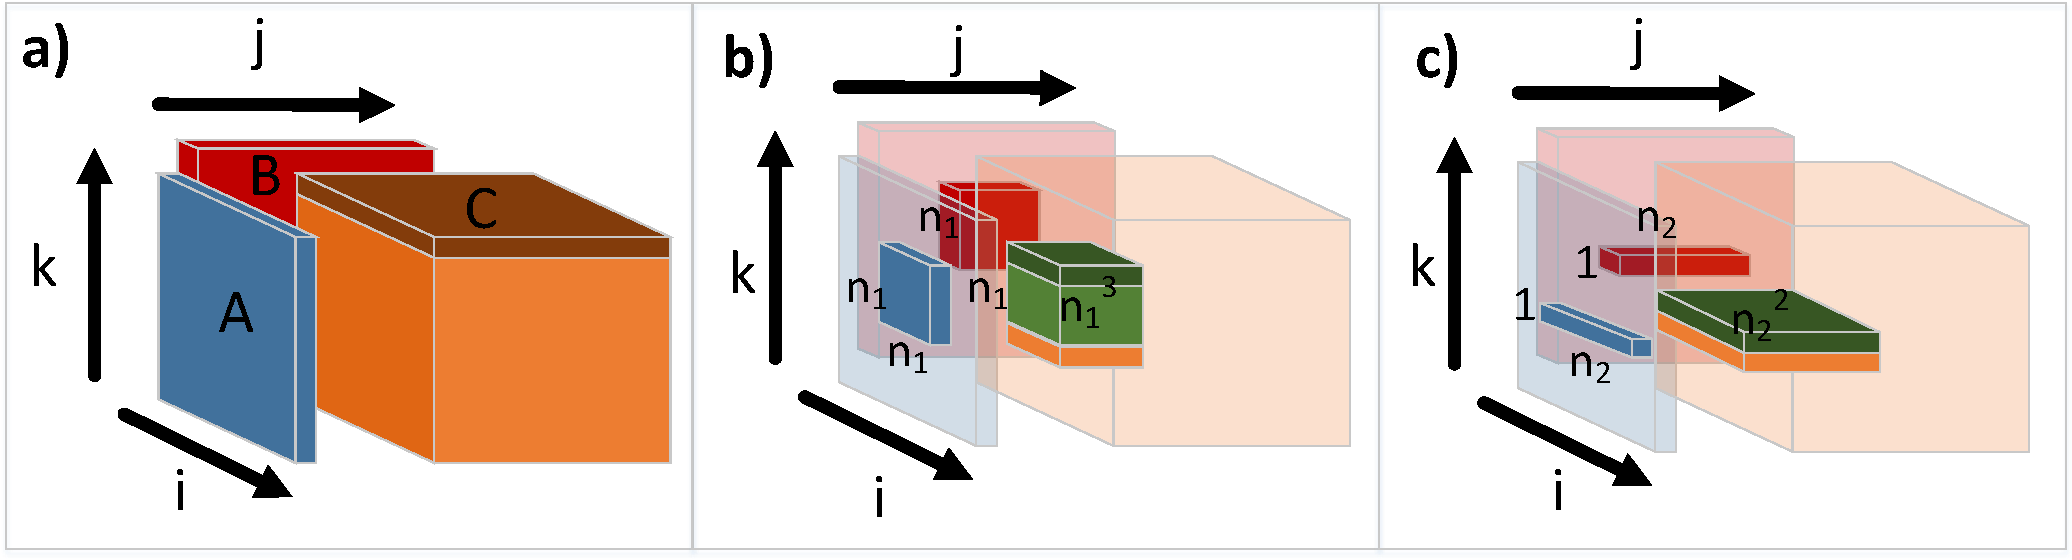
\includegraphics[width=\columnwidth]{figures/mmm_reuse}
%  \caption{MMM subset shape. a) 
%    geometric interpretation of $C = A B$ (orange cube represents 
%    3-dimensional iteration space of partial sums, matrix C is formed by 
%    reduction over dimension $k$ - represented by dark orange plane). b) 
%    optimal surface to volume subset shape. Note that in a subsequent 
%    subset computation only one of the three planes (blue, red or dark 
%    green) can be reused. c) the optimal subset shapes when 
%    data reuse is considered. In b) and c) blue, red, and orange surfaces 
%    form the dominator set, whereas dark green surface is the 
%    minimum set.}
%  \label{fig:mmmreuse}
%\end{figure}

To show why Lemma 2 gives a tighter bound than Lemma 1, consider a CDAG of 
MMM.  We can draw it in a 3D iteration space $\mathcal{V}$.
(\cref{sec:iterationSpace}, ~\ref{fig:iterationSpace}). Then,
an $S$-partition is a decomposition of this space into subcomputations $V_i$ 
whose
number of inputs ($|\alpha_i| + |\beta_i| + |\gamma_i|$) is smaller than $S$.
When a subcomputation is viewed as a subspace in the iteration space $V_i \in 
\mathcal{V}$, this input constraint may be viewed as a generalization of the 
Loomis-Whitney inequality~\cite{loomisWhitney}, which relates a cardinality of 
a 
finite set in $\mathbb{Z}^t$ with cardinalities of its projections to all $t$ 
dimensions. This technique was used by Irony et al.~\cite{loomisApplied} to 
derive first parallel I/O MMM lower bounds.

Assume that each subcomputation forms a cuboid $[a \times b \times c]$ in this
iteration space (we actually prove it in~\cref{sec:seqScheduling}). Its
faces form the dominator set.  Now based on Lemma~\ref{eq:redbluebound}, we 
construct a $2S$-partition with a
minimal cardinality, deriving subcomputations of a cubic ($a = b = c$) shape
(Figure~\ref{fig:iterationSpace} b), with a cube side $a = \sqrt{2S/3}$.  Such
schedule will perform $2a^2 \frac{n^3}{a^3} =
\sqrt{\frac{3}{2}}\frac{2N^3}{\sqrt{S}}$ I/O operations. 

Now, the question is: what is the size of a maximum reuse $R(S)$? Observe that
only one of three faces of this cuboid can be reused (used by a subsequent
subcomputation while still being in fast memory). This observation will help us
derive in (~\cref{sec:seqScheduling}) a "flat" shape (Figure 
\ref{fig:iterationSpace}
c) which performs $\frac{2N^3}{\sqrt{S}}$ I/O operations - an $\sqrt{3/2}$
improvement.


\section{\hspace{-0.5em}Optimal Sequential Matrix Multiplication}
\label{sec:seqOptimality}

We now proceed to establish a tight sequential I/O lower bound of MMM. Using 
the 
mathematical machinery of 
Lemma~\ref{lma:reuse}, we show a constructive proof of $Q \ge 2MNK/\sqrt{S} + 
MN$. This result has three main contributions (1) it is an additive 
improvement 
over the bound $2mnk/\sqrt{S} - 2S$ by Smith and van de Geijn~\cite{tightMMM} 
by an
additive factor of $2S + mn$, (2) the proof is constructive - what immediately 
follows is a corresponding schedule, (3) generality of a used technique is 
later used to derive I/O optimal parallel schedule~(\cref{sec:parOptimality}) 
and may be used in other 
linear algebra problems.
%
%\mac{the} I/O lower bound of MMM \mac{Now I'm confused, is it the
%new proof that is a new contribution, or the lower bound, or both? If the
%proof, then WHY does it matter that you have a new proof? What's the deep
%insight coming from this proof? And then why do you comment on tightening the
%bound (below), if it's just a proof? And if it's the bound that is the new
%contribution, then say it (underline it better!) and remove the ``new'' proof
%adjective. And if it's both, then just make this sound better here} \mac{add
%here ``, namely''} $Q \ge \frac{mnk}{\sqrt{S}} + mn$ \mac{,} and show a
%schedule achieving it. This result will be used in
%Section~\cref{sec:parOptimality} to prove tight bounds for parallel execution
%and a schedule that is \emph{independent of any combination of problem
%parameters} \mac{I would make this sentence the last in this paragraph}.
%%
%We derive \emph{all} constant terms improving the well-known asymptotic 
%results
%due to Hong and Kung~\cite{redblue} and Irony et al.~\cite{IronyMMM}, and
%tightening the bound $2mnk/\sqrt{S} - 2S$ by Smith and van de Geijn by an
%additive factor of $2S + mn$ \mac{I think it's better to place this sentence
%right after the sentence with the lower bound, to immediately justify why this
%new result matters}.
%
%\mac{Just in case, old beginning is below, commented}
%%   
%%   We now proceed to establish a key step to our main result. Using the 
%%   mathematical machinery of Lemma 2, we show a new proof of I/O lower bound 
%%of 
%%   MMM $Q \ge \frac{mnk}{\sqrt{S}} + mn$ and show a schedule achieving it. 
%%This 
%%   result will be used in Section~\cref{sec:parOptimality} to prove tight 
%%bounds 
%%   for parallel execution and a schedule 
%%   that is \emph{independent of any combination of problem parameters}.
%%   %
%%   We derive \emph{all} constant terms improving the well-known asymptotic
%%   results due to Hong and Kung~\cite{redblue} and Irony et 
%%al.~\cite{IronyMMM}, 
%%   and tightening the bound $2mnk/\sqrt{S} - 2S$ by Smith and van de Geijn by
%%   an additive factor of $2S + mn$.
%
%
%\greg{commented out the whole subsection Top-down vs bottom-up. It is 
%mentioned 
%in the intro and not needed here at all.}

%\subsection{Top-Down vs Bottom-Up}
%
%\mac{The title is a bit confusing... Maybe we can remove it completely}
%
%\mac{No, I would start differently - with stating our approach, underlying 
%what
%is the paper contribution! E.g., "We do bottom-top (see Figure X), as opposed 
%to [all
%others], [here is briefly why]}
%%
%Most of the current state-of-the-art algorithms, like Cannon's~\cite{Cannon},
%SUMMA~\cite{summa}, 3D SUMMA~\cite{summa3d}, or the 2.5D scheme~\cite{25d}
%use the "top-down" approach, that is, aim for decomposing the global domain
%evenly into $p$ processes (Figure \ref{fig:topdown-vs-bottomup}).
%%
%To obtain our schedule and prove its optimality, we use "bottom-up" approach,
%that is, defining the finest-granularity task for a single process and then
%identifying parallelization opportunities.  
%%
%\mac{Man, why do you provide this whole following part on task based
%programming?  What connection does it have? I would remove it completely, or
%move to a place where task based stuff is used...} 
%%
%Intuitively, the "bottom-up" approach shares similarities with task-based
%programming~\cite{taskparalelism}, which has also be used in the context of
%linear algebra~\cite{taskMMM}. The difference, however, is in the
%\emph{granularity}: A task is a single, I/O optimal, rank-1 \mac{rank-1 was 
%not
%defined} update (vector-vector outer product), instead of coarser grained
%rank-k \mac{rank-k was not defined} updates (matrix-matrix product) in
%recursive algorithms, like CARMA~\cite{CARMA}.
%%

%
%\subsection{Tight MMM Lower Bound}
%\label{sec:seqScheduling}
%
%
%\greg{commented out the whole beginning}
%\mac{Bad, you should provide some beginning in this paragraph}

%
%\mac{This title is too long}
%
%\mac{The following sequence is broken - how can algorithms
%derive their proofs? Moreover, ``derives'' should be ``derive'', right?}
%%
%"Top-down" algorithms, discussed in Section \ref{sec:seqOptimality}, 
%derives
%their 
%optimality proofs from maximizing computation to communication (input volume) 
%ratio.
%%
%\mac{At this point, I again think that it's bad because you start with 
%describing
%others, and not the stuff in this paper}
%The key difference between them, as well as the original lower bound lemma 
%(inequality 
%\ref{eq:redbluebound}) and the lemma presented in this paper (inequality 
%\ref{eq:reusebound}) is the explicit notion of reuse. \mac{The following 
%sentence
%sounds like a reasonable first sentence in this section...} In this section, 
%we prove 
%optimal sequential scheduling, \mac{The following sentence part is broken?} 
%which later be used to derive parallelization 
%strategies.
%%
%\mac{Why do I care? Underline ``what'' parallelization strategies you will
%obtain - optimal? near-optimal? faster than others? Make this announcement 
%(parallelization strategies)
%sounds more interesting... Also, strategies of what?} 
%%
%The crucial insight is that it is independent of matrix dimensions 
%and machine model (distributed or shared memory).
%%
%\mac{What? At this point I'm confused. You always wrote about this stuff 
%being 
%independent of
%problem parameters. But saying it's independent of machine model is extremely 
%confusing,
%considering the fact that you devoted so much space to describing I/O, etc 
%etc...}
%%
%\mac{In addition: ``it is independent of matrix dimensions
%and machine model'' is *not* a crucial insight... this is the advantage of
%this scheme. Insight is sth deep, some observation about the nature of 
%something.}
%%
%\mac{The following sentence: this is not a place for this... You should 
%discuss such
%things in related work. Sure, sometimes, one must discuss such connections 
%before
%related work, but make it concrete and to the point. Right now, you just say 
%`` We do X differently than others''. Why do I care? How does it help me 
%understand
%this section better?}
%%
%We use different technique than used by Smith and van de Geijn, who proved 
%sequential lower bound $2mnk/\sqrt{S} - 2S$ and prove a lower bound tighter 
%\mac{TIghter?
%Then why are we still better?} by 
%a constant factor of $2S$ :  $2mnk/\sqrt{S}$. Furthermore, the former result 
%does not count storing the output, which yields additional $mn$ I/O 
%operations.
%\mac{Again, at this point I read 15 lines of text in this *core* and *key* 
%section
%that should focus on describing your idea, and still I have no idea... more 
%than 30\%
%of this paragraph are some general notes, without obvious connection to the 
%flow of
%*this* section, about others' work. How should it help the reader understand 
%this
%section better?}
%
%\mac{The whole following part is again out of the place... I mean, shouldn't 
%it be
%explained in Background? How does it relate to the models from Background?}
%We use the computation model from Hong and Kung~\cite{redblue}, that is:
%\begin{enumerate}
%  \item A machine has a fast memory of size $S$ and a slow memory of infinite 
%  size,
%  \item all computations have to be performed inside fast memory, \mac{Huh?
%  But this sounds like you completely prevent *any* I/O during the execution?
%  So what's the point of I/O complexity anyway?}
%  \item at the beginning of computation, all inputs are in slow memory, and 
%  at the end of computation all the outputs must be stored back to slow 
%  memory. 
%\end{enumerate}
%

\begin{thm}[Sequential Matrix Multiplication I/O lower bound] 
	%Multiplying matrices of sizes $m \times k$ and $k \times m $ in the 
	%computation 
	%model from Definition~\ref{df:redbluegame} requires a minimum number of 
	%I/O 
	%operations is $\frac{mnk}{\sqrt{S}} + mn$.
	Multiplying matrices of sizes $m \times k$ and $k \times m $ requires a 
	minimum 
	number of $\frac{mnk}{\sqrt{S}} + mn$ I/O operations.
	\label{thm:seqlowbounds}
\end{thm}

\begin{proof}
	
	We first discuss a short intuition behind
	the proof. Next, we provide all details.
	
	\macb{Proof Intuition}
	%
	Using Lemma~\ref{lma:reuse}, we first establish a valid subset $V_i$ of an
	$S$-partition that achieves maximum computational intensity $\rho$ and find 
	its
	size (the number of vertices). Knowing $\rho$ and that there are $mnk$
	vertices in the whole MMM CDAG, we find the total
	I/O cost of the complete execution. Throughout the proof, in addition to
	full details, we include intuitive interpretations of key steps. To
	help keep up with the intuition, assume that $V_i$ is a 
	cuboid~(\cref{sec:iterationSpace}), and that we want to find its optimal 
	size 
	under certain conditions.
	
	%\greg{your comments are commented out}
	%  
	%\mac{It may be a good idea to first have a titled paragraph like here, with
	%the outline of the proof, followed by the (titled again) rest.}
	%%
	%We first derive a size \mac{Did you define precisely ``size of an 
	%S-partition?}
	%and shape \mac{``shape of an S-partition'' was clearly not defined before} 
	%of
	%an elementary \mac{What is ``elementary'' in this context? Again a 
	%confusing
	%word} S-partition subcomputation (subset) \mac{It seems these two words
	%(subcomputation, subset) mean the same thing? Use only one
	%consistently} $P$ that achieves 
	%maximum computational intensity $\rho$ \mac{I would explain briefly WHY 
	%you 
	%need
	%to derive this particular S-partition}. We then show the 
	%number of I/O operations per $P$ and derive the number of $P$ required to 
	%perform the whole computation. \mac{Again, I would briefly describe
	%the general intuition of the whole proof and the most important steps}
	
	\macb{Full Proof}
	%
	In this proof, we will use the iteration space 
	$\mathcal{V}$~(\cref{sec:iterationSpace}) to represent the 
	CDAG of MMM.
	By Definition~\ref{df:s-partition}, we divide the whole computation into
	$H(S)$ subcomputations $V_i, i \in \{1,\dots H(S)\}$, such that $Dom(V_i), 
	Min(V_i) \le 
	S$. As stated in~(\cref{sec:iterationSpace}), the dominator set of 
	$V_i$ is $Dom(V_i) =\phi_{ik}(V_i) \cup \phi_{kj}(V_i) \cup \phi_{ij}(V_i) 
	= 
	\alpha_i \cup \beta_i \cup \gamma_i$. Because all the read-after-write 
	(RAW) 
	dependencies are parallel to the vector~\textbf{k} (Line 5 in 
	Listing~1), the projection of the minimum set $Min(V_i)$ onto the plane 
	\textbf{ij} is also equal to $\gamma_i$ : ($\phi_{ij}(Min(V_i)) = 
	\gamma_i$).
	
	\textbf{Intuition:}  $\alpha_i, \beta_i$ and
	$\gamma_i$ are the faces of our cuboid $V_i$. The ``bottom'' face $\gamma_i$
	(Figure~\ref{fig:iterationSpace}) is formed by partial results of $C$ from
	previous subcomputations, and the ``top'' face is formed by partial results
	evaluated by $V_i$, also forming input for
	the next subcomputation. Because all the dependencies are facing 
	``upwards'', 
	the minimum set (the ``top'' face) is positioned directly above the 
	required 
	partial results of $C$, that is $\phi_{ij}(Dom(V_i)) = \phi_{ij}(Min(V_i))$.
	
	By the definition of $S$-partition, we have:
	
	\begin{gather}
	\label{eq:dm}
	|Dom(V_i)| = |\alpha_i| + |\beta_i| + |\gamma_i| \le S \\
	\nonumber
	|Min(V_i)| = |\gamma_i| \le S
	\end{gather}
	
	
	
	On the other hand, the Loomis-Whitney
	inequality~\cite{loomisWhitney} bounds the volume of $V_i$: 
	
	\begin{equation}
	\label{eq:lm}
	V_i \le \sqrt{|\alpha_i| |\beta_i| |\gamma_i|}
	\end{equation}
	
	
	%\textbf{Intuition:} Loomis-Whitney inequality bounds the volume of our 
	%cuboid
	%by the size of its faces.  \mac{I miss here some short text stating this
	%inequality and explaining how/why (formally) you can actually use it in our
	%context}
	
	Now we proceed to find the upper bound on the maximum reuse size $R(S) = 
	\max_{j = 1 \dots
		H(S)}(|V_{R,i}|)$. Consider two subsequent computations, $V_i$ and 
		$V_{i+1}$.
	Right after $V_i$, $\alpha_i$, $\beta_i$ and $\gamma_i$ may have red 
	pebbles on 
	them (they are in the fast memory). On the other hand the dominator set of 
	$V_{i+1}$ is $Dom(V_{i+1}) = \alpha_{i+1} \sum \beta_{i+1} \sum 
	\gamma_{i+1}$.
	Then, the reuse set $V_{R,i+1}$ is an intersection of those two sets:
	
	\begin{gather}
	\nonumber
	V_{R,i+1}
	\subset (\alpha_i \cup \beta_i \cup \gamma_i) \cap (\alpha_{i+1} 
	\cup 
	\beta_{i+1} \cup \gamma_{i+1}) \\
	\label{eq:vri1}
	= (\alpha_i \cap \alpha_{i+1}) \cup ( 
	\beta_i \cap 
	\beta_{i+1}) \cup (\gamma_i \cap \gamma_{i+1})
	\end{gather}
	
	\textbf{Intuition:}
	Visualizing $V_i$ and $V_{i+1}$ as two cuboids, they can only be positioned 
	in 
	the 3D space so that 
	they share at most one of their sides (either $\alpha_i \cap \alpha_{i+1} 
	\ne 
	\emptyset$ or  $\beta_i \cap \beta_{i+1} \ne \emptyset$ or  $\gamma_i \cap 
	\gamma_{i+1} \ne \emptyset$ ). If we allow other shapes than cuboids, 
	their shared surface is a sum of its projections into the three planes,  
	$\alpha_i \cap \alpha_{i+1}$,   $\beta_i \cap \beta_{i+1}$, and $\gamma_i 
	\cap 
	\gamma_{i+1}$.
	
	
	Note that $\alpha_i, \beta_i \subset \mathcal{I}$ are inputs of the 
	computation:
	therefore,
	by the Definition~\ref{df:redbluegame}, they start in the slow memory (they 
	already have blue 
	pebbles).
	$\gamma_i$, on the other hand, is the projection of the
	minimum set $\phi_{ij}(Min(V_i)) = \gamma_i$. Therefore, at the end of 
	$V_i$, 
	vertices in $Min(V_i)$ may have only red pebbles
	placed on them (they may have not been stored back to the slow memory yet). 
	Furthermore, by the Definition~\ref{df:s-partition}, these 
	vertices have children that have not been pebbled yet. 
	They either have to be reused forming the reuse set $V_{R,i+1}$, or
	stored back, forming $W_{BR,i}$ and requiring the placement of the blue 
	pebbles. 
	Because by their definition, $\gamma_i \cap \alpha_i = \gamma_i \cap 
	\beta_i = 
	\emptyset$, we have $\gamma_i \cap V_{R,i+1} =  \gamma_i \cap
	\gamma_{i+1}$ and $W_{BR,i} =  \gamma_i \setminus
	\gamma_{i+1}$. Then, the number of I/O operations $Q_i$ performed by the 
	subcomputation $V_i$ (cf. Lemma~\ref{lma:reuse}):
	
	\begin{equation}
	\label{eq:qi}
	Q_i \ge |Dom(V_i)| - |V_{R,i}| + |W_{BR,i}|
	\end{equation} 
	
	\textbf{Intuition:} The dominator set of each subcomputation consists of 
	certain
	elements from input matrices $A$ and $B$, as well as the partial results
	of $C$. The number of loads
	required by $V_i$ is the size of the dominator set $Dom(V_i)$ reduced by the
	elements already loaded (the reuse set $V_{R,i}$). The number of stores is 
	equal to the
	number of outputs $|\gamma_i|$  that are not reused in subcomputation 
	$V_{i+1}$, that is, 
	not contained in $|\gamma_{i+1}|$.
	
	We now proceed to find $\alpha_i, \beta_i$, and $\gamma_i$
	that maximizes the computational
	intensity $\rho_i = \rho$ (~\cref{sec:compIntensity}).
	We can bound $\rho_i$ by inserting Equations~\ref{eq:dm}, \ref{eq:lm}, 
	~\ref{eq:vri1} and~\ref{eq:qi}:
	
	\begin{gather}
	\nonumber
	\rho_i = \frac{|V_i|}{|Dom(V_i)| - |V_{R,i}| + |W_{BR,i}|} \\
	\nonumber
	\le 
	\frac{\sqrt{|\alpha_i||\beta_i||\gamma_i|}}{|\alpha_i| + |\beta_i| + 
		|\gamma_i| - |\gamma_i \cap \gamma_{i+1}| +  |\gamma_i \setminus 
		\gamma_{i+1}|}
	\end{gather}
	
	We immediately see that to maximize $\rho_i$, we have $\gamma_{i+1} = 
	\gamma_i$, as it both maximizes $|\gamma_i \cap 
	\gamma_{i+1}|$ and minimizes $|\gamma_i \setminus \gamma_{i+1}|$.
	
	We then formulate it as an 
	optimization problem:
	
	%Inserting Equation~\ref{eq:vri1} to~\ref{eq:qi} we see that to minimize 
	%$Q_i$ 
	%we have $\gamma_{i+1} = \gamma_i$, as it both maximizes $|\gamma_i \cap 
	%\gamma_{i+1}|$ and minimizes $|\gamma_i \setminus \gamma_{i+1}|$, while 
	%$|Dom(V_i)|$ does not depend on the choice of $\gamma_{i+1}$.
	%
	%
	%W.l.o.g., assume that the subcomputation $V_i$ 
	%achieves the maximum computational
	%intensity $\rho_i = \rho$ (~\cref{sec:compIntensity}). To
	%find $\alpha_i, \beta_i$ and $\gamma_i$, we formulate it as the 
	%optimization 
	%problem:
	
	
	
	%\begin{multline}
	%\\
	%\text{maximize } \rho = \frac{|V_i|}{|Dom(V_i)| - |V_{R,i}| + |W_{BR,i}|} 
	%\\
	%\text{subject to: } |Dom(V_i)| \le S \\
	%\end{multline}
	
	\begin{multline}
	\\
	\text{maximize }
	\sqrt{\gamma_i}\frac{\sqrt{|\alpha_i| |\beta_i|}}{|\alpha_i| + |\beta_i|}\\
	\text{subject to: } \\
	|Dom(V_i)| = |\alpha_i| + |\beta_i| + |\gamma_i| \le S \\
	|\alpha_i|, |\beta_i|, |\gamma_i| \in \mathcal{Z} 
	\end{multline}
	
	Observe that to maximize $\frac{\sqrt{|\alpha_i| |\beta_i|}}{|\alpha_i| +
		|\beta_i|}$ we have $|\alpha_i| = |\beta_i|$. Then the solution to this
	maximization problem gives  $|\alpha_i| = |\beta_i| \rightarrow 0$, 
	$|\gamma_i|
	\rightarrow S$. But because $\alpha_i$, $\beta_i$ and $\gamma_i$ are sets 
	of 
	vertices, therefore $|\alpha_i|, |\beta_i|, |\gamma_i| \in \mathcal{Z}$.
	Furthermore, we have $\phi_{kj}(\alpha_i) =
	\phi_{ik}(\beta_i)$, $\phi_{ij}(\alpha_i) = \phi_{ik}(\gamma_i)$ and
	$\phi_{ij}(\beta) = \phi_{kj}(\gamma)$. Finally, we get:
	
	\begin{multline}
	\label{eq:seqSolution}
	\\
	|\alpha_i| = |\beta_i|= \left \lfloor{\sqrt{S + 1} - 1} \right \rfloor \\
	|\phi_{kj}(\alpha)| = |\phi_{ik}(\beta)| = 1 \\
	|\gamma| = |\alpha| |\beta| = \left \lfloor{(\sqrt{S + 1} - 1)^2} \right 
	\rfloor 
	\\
	\end{multline}
	
	
	
	From now on, to keep the calculations simpler, we use the following 
	approximation:
	
	\begin{equation}
	\label{eq:approx}
	\left \lfloor{\sqrt{S + 1} - 1} \right \rfloor \approx \sqrt{S}
	\end{equation}
	
	All the following results may be easily rewritten using the precise formula 
	and
	are correct up to this approximation factor.
	
	Using the approximation~\ref{eq:approx}, we have $|V_i| = S, R(S) = V_{R,i} 
	= 
	|\gamma_i| = S, \rho =
	\sqrt{S}/2$.
	Finally,  by Corollary \ref{cor:q}:  
	$$Q \ge
	\frac{|V|}{\rho} = \frac{2mnk}{\sqrt{S}}$$ 
	This is the I/O cost of putting a red pebble at least once on every vertex 
	in 
	$\mathcal{V}$. Note however, that we did not put any
	blue pebbles on the outputs yet (all vertices in $\mathcal{V}$ had only red
	pebbles placed on them during the execution). By
	Definition~\ref{df:redbluegame}, we need to place blue pebbles on $mn$ 
	output
	vertices, corresponding to the output matrix $C$, resulting in additional 
	$mn$
	I/O operations, yielding final bound
	$$Q \ge \frac{2mnk}{\sqrt{S}} + mn$$ 
	%
\end{proof}

\subsection{I/O Optimal Schedule}
\label{sec:seqScheduling2}

The proof of Theorem~\ref{thm:seqlowbounds} is constructive:
that is, from it we immediately obtain a schedule achieving it. The optimal
subcomputation $V_i$ corresponds to $S$ calculated partial products of C. Its
inputs $\alpha$ and $\beta$ are subsets of a single column of $A$ and a single
row of $B$, both of length $\sqrt{S}$. This may be viewed as an outer product
formulation of MMM: each subcomputation is an outer product of two vectors of
length $\sqrt{S}$, with subsequent subcomputations updating this result
(Listing~\ref{lst:pseudocode}).

\begin{lstlisting}[float=h, caption=Pseudocode of I/O optimal sequential MMM, 
label=lst:pseudocode]
T = $\sqrt{S}$
for i_1 = 1:m/T
	for j_1 = 1:n/T
		for r = 1:k    % k is the outer loop
			%elementary subcomputation V
			for i_2 = i_1*T : (i_1+1)*T
				for j_2 = j_1*T : (j_1+1)*T
					C(i_2,j_2) = C(i_2,j_2) + A(i_2,r)*B(r,j_2)
				end for
			end for 
		end for
	end for 
end for
\end{lstlisting}
%
%We note that an implementation based on this outer
%schedule is the Goto algorithm~\cite{Goto}. 

%-------------old version starts here----------%
%\greg{------------old version starts here -----------} 
%
%
%
%Let's \mac{Let's is too informal} represent the matrix multiplication 
%operations \mac{What are ``matrix multiplication operations''?
%again, confusing. Intuitively it may be clear, but this must be precise. The 
%actual products of matrix elements? the sums? more precision} as the three 
%dimensional 
%iteration space \mac{This is much more your domain and not main, but 
%``iteration space'' also
%sounds quite vague}. Let $i,j,k$ be dimensions corresponding to matrix sizes 
%$m,n,k$, that is, matrix $A$ lays on the plane $ik$, matrix $B$ lays on the 
%plane $kj$ and matrix $C$ lays on the plane $ij$ \mac{This again is somewhat 
%confusing. What is ``plane'' mathematically here?
%This is proof, all must be clear. Define plane... But then I know, there are 
%many
%of these concepts (as we discussed while hiking), and defining them all
%would be very tedious... My recommendation - \ul{I suggest you read several
%proofs from top math conferences related to this type of things, and see how 
%people deal with this}}.
%
%\mac{\ul{Another important comment:} at this point, it becomes clear that
%the paper lacks some background into the MM stuff. I mean, you need to
%lay out the setting... All these MM-related concepts such as laying matrices
%A, B, C onto different ``planes of computation'' must be introduced in
%Background.}
%%
%Assume that the searched subset \mac{I would use some symbol for this subset
%that maximizes intensity} computes $\mathcal{V}$ partial products $c = c + ab$
%\mac{what? why $c = c + ab$? Mathematically, unless $ab=0$, it's never true,
%right?} of $C$ \mac{\ul{First comment:} Also, it's confusing: what are
%``products of $C$''??}. Then, the projection of $\phi_{ik}(\mathcal{V})$
%\mac{``Projection'' was never defined (extremely confusing). \ul{Second
%comment:} Moreover: what is this $\mathcal{V}$? it is also not defined. In the
%sentence before, it sounds like a number (``$\mathcal{V}$ products''), but 
%here
%it sounds more like something more complex than a number? Again confusing.
%\ul{Third comment}: is it "the projection of" OR "the projection"? It makes a
%huge difference. Now it sounds like it should be "the projection" (and is
%wrongly "the projection of"} onto plane $ik$ correspond \mac{``corresponds''
%instead of ``correspond''?} to the required inputs from $A$.  \mac{Very
%confusing - WHY does this projection correspond to the input? It will be
%unclear to the reader... Maybe with the proper background it will clarify?}
%Let's \mac{Let's is informal - better just "Denote"} denote $A$'s input
%$\phi_{ik}(\mathcal{V}) = \alpha$ \mac{Symbol for denote should be different
%from $=$, I would just use a word ``as''}.  Similarly, $\phi_{kj}(\mathcal{V})
%= \beta$ and $\phi_{ij}(\mathcal{V}) = \gamma$, which correspond to partial
%results of $C$ being updated \mac{This part of sentence is again extremely
%confusing. What partial results? Why? You just wrote about some inputs, why
%suddenly something corresponds to some partial results of $C$?  and what does
%it mean ``$C$ being updated''? How updated?}. Furthermore, note that $\gamma$
%is also the output of the subcomputation \mac{what ``subcomputation''?  In the
%context of S-partitions? Or is it something purely MM-related?  If yes, what
%exactly? Adding one element to one element of $C$? computing a block of $C$?
%what?}, as those inputs are updated \mac{How updated? Confusing again...}.
%
%To compute $\mathcal{V}$ partial products $c = c + ab$ of $C$ \mac{Same
%comments as before, it's confusing on that these symbols really mean. \ul{I
%mean, the point is that to someone who is specializing in MM stuff, this will
%more or less be somewhat clear}: c = c + ab will mean that you update some
%element of C with corresponding ab. However, ANY OTHER person will be lost
%after the FIRST SENTENCE of this section / proof. In addition, even if a
%reviewer related to MM understands the stuff, it will not help in persuading
%him/her to accept the paper, because they will notice all these confusing
%parts}, we need $\alpha$ and $\beta$ elements of matrices $A$ and $B$
%\mac{What are precisely these elements of matrices?} and $\gamma$ elements of
%$C$, corresponding to the updated values of $c$ (Figure \ref{fig:mmmreuse})
%\mac{This sentence before is also confusing with respect}.  Therefore, the
%input size \mac{What is ``input'' in this current context?} (surface in
%geometric interpretation \mac{You never defined anything related to the
%geometric interpretation}) is $\mathcal{I} = |\alpha| + |\beta| + |\gamma|$
%\mac{This equality is unclear - not obvious why it should be true}. According
%to the definition of S-partition, $$\mathcal{I} = |\alpha| + |\beta| +
%|\gamma|\le S$$ \mac{This previous inequality is important - it combines MM 
%and
%I/O complexity...  But it's also unclear why this is the case. This must be
%explained more extensively / appropriately}.  From Loomis-Whitney inequality
%\cite{loomisWhitney}, we have the upper bound on $$\mathcal{V} \le
%\sqrt{|\alpha| |\beta| |\gamma|}$$ \mac{I would consider putting 1-2 sentences
%on the Loomis-Whitney stuff... maybe}.  The upper bound on te \mac{the?} reuse
%$R(S)$ \mac{At this point, no idea what R(S) is. It was defined, but it gets 
%so
%complex at this stage that readers won't know. I suggest to remind somehow 
%what
%it is, intuitively. \ul{Another suggestion: MAYBE a solution to the whole
%problem of the complexity is to, like I guess we already discussed, is to 
%start
%early in background with matrix multiplication, and then, at every step of the
%I/O stuff, provide relations to MM. THis way, people will always get these two
%next to each other in their minds}} is a largest \mac{The largest?} projection
%of $\mathcal{V}$ to any surface $\mathcal{P}$ in the $ijk$ space \mac{To an
%arbitrary one? Or to one of the 3 ``canonical'' ones?}: $$R(S) \le
%\max_\mathcal{P}(|\phi_\mathcal{P}(V)|)$$ \mac{What is the definition of the 
%$|
%\cdot |$ symbol above in the current context?} Furthermore $\alpha$ and 
%$\beta$
%are the inputs and do not need to be stored \mac{Really? Why not? AN average
%reader will think it's not true, because you always must store input 
%somewhere?
%Make it precise what it means (no I/O)?}.  $\gamma$, on the other hand, is the
%set of partial results and either has to be reused or stored, increasing the
%I/O cost \mac{What is precisely ``I/O cost''? I know, I know, that's all what
%the paper is about, but I think it might not hurt to clearly state / define at
%the very beginning some cost function for this thing...}. 
%
%Let's \mac{Informal} denote $\alpha_i$ and $\beta_i$ as inputs of $i$-th
%subcomputation \mac{What is ith subcomputation? How does it relate to the I/O
%business? Confusing, not clear}, $\gamma_i$ as its input and output, and $R_i$
%as its reuse (subset of inputs that is already in the fast memory \mac{Why do
%you suddenly remind HERE what reuse is, and did not do this several lines
%above?}). Then, $$R_i = (\alpha_i \cap \alpha_{i-1}) \cup (\beta_i \cap
%\beta_{i-1}) \cup (\gamma_i \cap \gamma_{i-1}) $$ \mac{This series of unions 
%is
%unclear} Note that $|\gamma_i \setminus \gamma_{i+1}|$ outputs have to be
%stored back to the memory \mac{why?}. The I/O cost of $i$-th subcomputation is
%$$Q_i = |\mathcal{I}| - |R_i| + |\gamma_i \setminus \gamma_{i+1}|$$.
%
%The projection plane $\mathcal{P}$ \mac{What is ``projection plane''?}
%minimizing $Q_i$ \mac{What does it mean ``minimizing'' in the current context?
%meaning, it's not fully clear what the connection between planes and
%minimization is} is therefore $\mathcal{P} = ij$, resulting in $\gamma_i =
%\gamma_{i+1}$\mac{What does this last equality intuitively mean?}. 
%Intuitively,
%this is clear that we should reuse partial results of $C$ immediately, instead
%of storing them back to the memory. Therefore, to obtain the optimal
%subcomputation, we formulate it as the optimization problem \mac{``Therefore''
%- it is not clear why ``formulating it as an optimization problem'' is a
%logical consequence of the previous sentence}:
%
%\begin{multline}
%\\
%\text{maximize } \rho = \frac{|\mathcal{V}|}{\mathcal{I} - |R|} \le 
%\frac{\sqrt{|\alpha| |\beta| |\gamma|}}{|\alpha| + |\beta|}\\
%\text{subject to: } |\alpha| + |\beta| + |\gamma| \le S \\
%\end{multline}
%
%Exploiting the symmetry of the domain \mac{What is ``the symmetry of the
%domain''?} by plane \mac{What does it mean ``by plane'' in this context?}
%\textbf{(i + j)k} \mac{Why bold now and not before?}, we have  $|\alpha| =
%|\beta|$. Now the solution to this problem gives $|\alpha| = |\beta|
%\rightarrow 0$, $|\gamma| \rightarrow S$ \mac{Unclear how you get these
%results}.  Restricting the solution to the integer lattice ($\alpha, \beta,
%\gamma \in \mathbb{Z}$) we get the optimal shape of the subcomputation
%\mac{Again, this shape of subcomputation should be more clear}:
%
%\begin{multline}
%%\label{eq:seqSolution}
%\\
%|\phi_{ij}(\alpha)| = |\phi_{ik}(\alpha)|  = |\phi_{ij}(\beta)| = 
%|\phi_{kj}(\beta)|= \sqrt{S + 1} - 1 \\
%|\phi_{kj}(\alpha)| = |\phi_{ik}(\beta)| = 1 \\
%|\gamma| = |\alpha| |\beta| = (\sqrt{S + 1} - 1)^2 \\
%\end{multline}
%
%This corresponds to a single column of $A$ and row of $B$ of length $\sqrt{S +
%1} - 1$ and a square subset of $C$ of $(\sqrt{S + 1} - 1)^2$.  \textbf{From 
%now
%on, to keep the notation \mac{It's not notation that you keep simpler here,
%it's calculations?} simpler, we approximate} 
%\begin{equation}
%\label{eq:approx}
%\sqrt{S + 1} - 1 \approx \sqrt{S}
%\end{equation}
%All the following results may be easily rewritten using the precise formula 
%and
%are correct up to this approximation factor.
%
%
%This result immediately gives $\mathcal{V} = S, R(S) = S, \rho = \sqrt{S}/2$
%\mac{How do you get these? Completely unclear} and finally, according to
%corollary \ref{cor:q}:  $Q \ge \frac{|V|}{\rho} = \frac{2mnk}{\sqrt{S}}$. This
%is only the input cost \mac{Huh? What is the input cost? Why input cost?}, as
%for now, we assumed that all the outputs were reused. However, $mn$ outputs
%  have to be stored back to the memory, yielding additional $mn$ I/O 
%operations
%  \mac{Unclear sentence}. 
%
%%-------------old version ends here----------%
%\greg{------------old version ends here -----------} 

\bibliographystyle{ACM-Reference-Format}
\bibliography{mmm-ppopp}



\end{document}
